%!TEX root = ../thesis_a4.tex

\chapter{Background}
\label{chap:background}

\section{Introduction}

In this chapter, we present our review of the existing literature on research topics related with the work presented in this thesis. In addition, we also present an overview of the relevant music and scientific background. We start with a brief discussion on the terminology used in this thesis (\secref{sec:background_terminology}). Subsequently, we provide an overview of the selected music concepts to better understand the computational tasks addressed in our work (\secref{sec:music_background}). We then present a review of the relevant literature, which we divide into two parts. We first present a review of the work done in computational analysis of \gls{iam} (\secref{sec:background_relevant_work_iam}). This includes approaches for tonic identification, melodic pattern processing and automatic \gls{raga} recognition. In the second part, we present relevant work done in \gls{mir} in general on topics closely related with pattern processing (detection and discovery), and key estimation (\secref{sec:background_relevant_work_other_music}). Finally, we provide a brief overview of selected scientific concepts (\secref{sec:background_scientific_background}).% To conclude the chapter, we provide a summary of the literature review, wherein we highlight the shortcomings of the existing approaches, and identify some possible venues for scientific contribution (\secref{sec:background_summary}). 

%Finally, we provide a brief overview of selected scientific concepts in information retrieval, time-series analysis, complex networks and statistics (\secref{sec:background_scientific_background}). 


\section{Terminology}
\label{sec:background_terminology}

In this section, we provide our working definition of selected terms that we have used throughout the thesis. To begin, it is important to understand the meaning of melody in the context of this thesis. As we see from the literature, defining melody is in itself has been a challenge, with no consensus on a single definition of melody~\citep{gomez2003melody,salamon:phd:13}. We do not aim here to formally define melody in an universal sense, but present its working definition within the scope of this thesis. Before we proceed, it is important to understand the setup of a concert of \gls{iam}. Every Performance of \gls{iam} has a lead artist, who plays the central role (also literally positioned in the center of the stage), and all other instruments are considered as accompaniments. There is a main melody line by the lead performer, and typically, also a melodic accompaniment that follows the main melody. A more detailed description of the concert setup in \gls{iam} is provided in~\secref{sec:music_background}. Since \gls{iam} is a predominantly a performance-based music tradition, even the studio recordings and the released commercial music follow the same setup.

In the context described above, merging relevant parts of the definitions given by~\cite{paiva2006melody} and~\cite{levitin2002memory} covers to a large extent the scope of melody in \gls{iam} from a computational point of view. These definitions are:

\blockquote[\cite{paiva2006melody}]{``\textit{the dominant individual pitched line in a musical ensemble}''}

\blockquote[\cite{levitin2002memory}]{``\textit{an auditory object that emerges from a series of transformations along the six dimensions: pitch, tempo, timbre, loudness, spatial location, and reverberant environment}''}

The first definition falls short of considering several other dimensions of sound such as timbre and loudness that are important in perception and production of melody, which are taken into account in the second definition. The concept of audio as a mixture of sounds from multiple instruments (`\textit{ensemble}') is missing in the second definition. The idea of continuity and smoothness of melody is expressed by `\textit{line}' in the former and by `\textit{series of transformations}' in the latter. Combining these two definitions we obtain our working definition as: 

\blockquote{\textit{an auditory object that emerges from a continuous series of transformations along the six dimensions: pitch, tempo, timbre, loudness, spatial location, and reverberant environment, by the dominant individual melodic source in a music ensemble}}. 

Though our definition of melody considers several dimensions of sound, for computational purposes we use a low-level representation of melody that only describes the pitch dimension of sound. We represent melody by a continuous pitch time-series corresponding to the lead artist in an audio recording, also referred to as predominant pitch in the subsequent chapters. In \gls{mir} it is also commonly referred to as predominant melody. 

We now proceed to define the terms such as melodic patterns, phrases and motifs. It is important to disambiguate them with other seemingly synonymous terms such as melodic fragment and segment. Melodic fragment and segment in this thesis refer to a continuous time region in melody (essentially a pitch subsequence). Both these terms do not entail any musical connotation and are used synonymously in this document. On the other hand, by a melodic pattern we refer to a recurring melodic fragment, wherein the scope and the meaning of repetition is contingent on the perceived melodic similarity by expert listeners in \gls{iam}.  Terms such as melodic patterns, fragments and segments thus refer to temporal units in our low-level representation of melodies. The term melodic phrase on the other hand is used in the context of music, as being a unit of melody that encapsulates an idea or a musical thought by an artist. However, even this term does not necessarily imply the phrase being characteristic of a \gls{raga}. To denote the characteristic phrase of a \gls{raga} we specifically use the term `\textit{characteristic}' along with melodic phrase, or at times simply denote by the term \gls{raga} motif. 

The term polyphonic audio in the context of music recordings in our work basically signifies that the recordings comprise a mixture of multiple instruments played simultaneously. It does not mean that the music or melody is polyphonic (functional polyphony) as understood in the context of Western classical music.

\section{Music Background}
\label{sec:music_background}

In this section, we provide a brief introduction to \gls{iam}, which is the tradition that we consider for the computational analysis in this thesis. We first briefly describe the general aspects of this  music tradition, and subsequently, provide a short introduction to the musical concepts related with the melodic aspects. Note that the description provided here is not comprehensive, and it is essentially to facilitate the understanding of the subsequent chapters. For a deeper understanding of these concepts we provide additional references wherever needed. 

\subsection{Indian Art Music}
\label{sec:music_background_iam}

In our work, \acrfull{iam} refers to two art music traditions of the Indian subcontinent; Hindustani music, also known as North Indian music~\citep{Bor2010, Danielou2010}, prominent in the northern and central regions of India, Pakistan, Nepal, Afghanistan and Bangladesh; and Carnatic music, widespread in the southern regions of the Indian subcontinent (South India and Srilanka)~\citep{Singh1995,Viswanathan2004}. \gls{iam} is also commonly referred to as \gls{icm}. Throughout the thesis we use the term ``art'' instead of ``Classical'' to refer to these music traditions. \cite[p. 1]{Raja2012} presents an interesting argument emphasizing the appropriateness of such a terminology. To give a brief historical perspective, the roots of \gls{iam} can be traced back to \gls{samved}, which is one of the four \gls{vedas} that describes music at length~\citep{Trivedi2008,Singh1995}. The \gls{samved} dates back to around 1000 BC, consists of a collection of religious hymns (taken from \gls{rigved}), to be sung using specifically indicated melodies called as \gls{samagan}~\citep{Griffith2004}. However, the current form of \gls{iam} is a confluence resulting from the cultural interactions between the Persian, Greek, Arabic, Iranian and Indian cultures~\citep{Kaul2007,Saraf2011,Singh1995}.

With its long existing history, \gls{iam} continues to thrive in diverse sociocultural contexts in both inside and outside India. There is an active audience base, and several music festivals such as Sawai Gandharva Bhimsen Mahotsav\footnote{http://sawaigandharvabhimsenmahotsav.com/} and Madras Music Season\footnote{http://www.musicacademymadras.in/} that exclusively feature these art music traditions. Notably, Madras Music Season is also one of the largest music festivals in the world that organizes more than 1500 individual artist concerts in a span of six weeks. \Gls{iam} is a well studied music tradition with sophisticated and grounded music theory. It has a substantial musicological literature and scholarly text written on different musical concepts. 

Over the centuries \gls{iam} has been orally transmitted across generations, following a hierarchical model of music training such as \gls{gharana} (or school of music) in Hindustani music~\citep{Saraf2011,Mehta2008}. Though the fundamental musical concepts used across \glspl{gharana} are the same, each \gls{gharana} has its own ideology and characteristic style of music performance~\citep{Deshpande1989}. 

Both Hindustani and Carnatic music are performance oriented music traditions, and are mainly improvisatory in nature. In Carnatic music, a concert, also referred to as Kach\={e}ri, is the natural unit of music performance. It is the unit typically considered for organization and digital distribution of Carnatic music content. A concert of Carnatic music typically comprises around 10 music pieces. Though Carnatic music is improvisatory in nature, the performances are based on compositions. Most of the compositions are to be sung, as a result of which, vocal music is dominant in Carnatic music. Even in instrumental music, artists aim to mimic vocal singing~\citep{Viswanathan2004}. In Hindustani music, individual music pieces tend to be long in duration (one single piece can last up to an hour). A concert typically contains a handful of such pieces. Vocal music is dominant in Hindustani music as well. However, compared to Carnatic music instrumental performances in Hindustani music are much more prevalent. 

We now describe the performance setup in \gls{iam}, which also gives us an idea about the characteristics of the recorded acoustic signal. \gls{iam} is essentially heterophonic in nature, with a main melody being sung or played by the lead artist~\citep{Bagchee1998}. Quintessentially, an instrument provides melodic accompaniment and follows the melody of the lead performer~\citep{Viswanathan2004}. A typical arrangement in a performance of Indian art music consists of a lead performer (in rare cases a duo), a rhythm accompaniment generally provided by \gls{tabla} in Hindustani music and \gls{mridangam} in Carnatic music, a constantly sounding drone in the background, and frequently, a melodic accompaniment using harmonium or \gls{sarangi} in Hindustani music and violin in Carnatic music. The drone sound which is mainly produced by a \gls{tanpura} is the only component that adds a harmonic element to the performance~\citep{Bagchee1998}. %In case of the instrumental Hindustani music, the prominent lead instrument are \gls{sitar}, \gls{sarod}, \gls{bansuri}, \gls{sarangi} and \gls{santur}.

Due to a wider geographical spread over the Indian subcontinent, Hindustani music is much more diverse and heterogeneous compared to Carnatic music. There are several forms and styles within this music tradition such as \gls{dhrupad}, \gls{khayal}, and \gls{thumri}. These forms differ considerable from each other and are characterized based on their singing styles and instrumentation~\citep{Bor2010}. In this thesis, we primarily focus on the \gls{khayal} form, which is currently one of the most frequently performed forms in Hindustani music. 

Despite a number of significant differences between Hindustani and Carnatic music, they share similar musical concepts. In both these music traditions \gls{raga} (often pronounced as r\={a}g in Hindustani music) is the melodic framework, and \gls{tala} (often pronounced as t\={a}l in Hindustani music) is the rhythmic framework. For the rest of this document we will use the terms \gls{raga} and \gls{tala} to denote these concepts for both the music traditions. Since this thesis focuses on the melodic aspects of \gls{iam}, we provide a brief overview of the \gls{raga} concept in the subsequent section. We also provide a short explanation of melody related terminology commonly used in \gls{iam}. 


\subsection{Melody in Indian Art Music}
\label{sec:melody_in_iam}

Melodies in \gls{iam} are based on the framework of \gls{raga}. It is one of the core musical concepts in \gls{iam} used in composition, performance, music organization, and pedagogy~\citep{Bagchee1998,Danielou2010}. Numerous compositions in Indian folk and film music are also based on \gls{iam}~\citep{ganti2013bollywood}.

Musicological literature on \gls{iam} is replete with explanations and definitions of \gls{raga}. Some of the interesting ones are as follows.

\blockcquote[p. 96]{martinez2001semiosis}{``\textit{The \gls{raga} is more fixed than a mode, and less fixed than the melody, beyond the mode and short of melody, and richer both than a given mode or a given melody.}''}

Which closely relates to

\blockcquote[]{powers1963background}{``\textit{A \gls{raga} is not a tune, nor is it a `modal' scale, but rather a continuum with scale and tune as its extremes.}''}

A more concrete definition specifically from an analytical point of view is given by;

\blockcquote[]{chordia2013joint}{``\textit{A \gls{raga} is most easily explained as a collection of melodic gestures, along with techniques for developing them. The gestures are sequences of notes that are often inflected with various micro-pitch alterations and articulated with an expressive sense of timing. Longer phrases are built by joining these melodic atoms together.}''}

Overall, we see that a \gls{raga} being more than a scale, mode and a discrete note sequence is highlighted in all the definitions. For computational modeling of melodic aspects in \gls{iam}, the definition of \gls{raga} given by~\cite{chordia2013joint} appears appropriate. Another way to comprehend the concept of \gls{raga} is to understand the aspects or properties that characterize \glspl{raga} such as the set of \glspl{svara}, \gls{arohana}-\gls{avrohana}, calan and its characteristic melodic phrases. A brief description of these different melodic aspects is provided in the subsequent paragraphs. For a more comprehensive description of these concepts we refer to~\citep{Danielou2010,Bagchee1998,Viswanathan2004}.

\COMMENT{Image of tonic, svaras, aroh-avroh, phrase, chalan,gamaka?}

\paragraph{Svaras:} The seven solfege symbols (Sa, Re, Ga, Ma, Pa, Dha and \acrshort{ni}, in short-forms) used in \gls{iam} are termed as \textit{svaras}~\citep{Danielou2010,Bagchee1998}. Except Sa and Pa (the fifth scale degree with respect to base \gls{svara} Sa), every other \gls{svara} has two or three variations. Every \gls{raga} comprises a set of typically five to seven \glspl{svara}. Each of these \glspl{svara} has a well defined function role in the context of a given \gls{raga}~\citep{Viswanathan2004}. \Glspl{svara} in a \gls{raga} are structured hierarchically, where the \gls{vadi} and the \gls{samvadi} \glspl{svara} are the first and the second most prominent \glspl{svara} in a melody. There are more functional roles such as a \gls{nyas} \gls{nyas} discussed in the subsequent paragraphs. 

\paragraph{Tonic pitch:} The concept of tonic is fundamental to the melodic structures in \gls{iam} \citep{Viswanathan2004,Danielou2010}. It is the base pitch of a performer, carefully chosen in order to explore the full pitch range effectively in a given \gls{raga} rendition. In a performance of \gls{iam}, tonic pitch is constantly reinforced by the drone sound in the background that is typically generated by the \gls{tanpura}. It acts a reference and the foundation for the melodic integration throughout the performance~\citep{Deva1980}. All the tones in the musical progression are constantly referred and related to the tonic pitch. All the accompanying instruments such as the \gls{sarangi}, violin, \gls{tabla} and \gls{mridangam} are tuned using the tonic of the lead performer. It should be carefully noted that tonic pitch in \gls{iam} refers to a particular pitch value and not to a pitch-class. The frequency range of the tonic pitch for male and female singers spans more than one octave, roughly 100-260\,Hz~\citep{Sengupta2005b}. In any performance of \gls{iam} the tonic pitch is the Sa (short-form of \gls{shadja}) \gls{svara} around which the \gls{raga} is built upon~\citep{Danielou2010,Bagchee1998}. Other set of \glspl{svara} used in the performance derive their meaning and purpose in relation to this reference, and to the specific tonal context established by the given \gls{raga}~\citep{Deva1980}. 

\paragraph{\titlecap{\glsentrytext{nyas}}:} \cite{Dey2008} presents various interpretations and perspectives on the concept of \gls{nyas} in Hindustani music according to ancient, medieval and modern authors. In the context of the current form of Hindustani music, the author describes \gls{nyas} as that process in a performance of a \gls{raga} where an artist pauses on a particular \gls{svara}, in order to build and subsequently sustain the format of a \gls{raga}~\citep[p. 70]{Dey2008}. The set of \glspl{svara} on which the pause is permitted in a \gls{raga} grammar are referred to as \gls{nyas} \glspl{svara}. Every \gls{raga} comprises a set of \glspl{svara} where an artist can momentarily pause to release the musical tension built in the melody. Dey further elaborates the concept of \gls{nyas} in terms of action, subject, medium, purpose and effect associated with it. Typically, occurrence of a \gls{nyas} \glspl{svara} mark the ending of a melodic phrase. A \gls{nyas} is mostly manifested in a melody as a long held \gls{svara}. However, there are several exceptions to it, which mainly depend on the local melodic context and the global tonal context defined by the \gls{raga}. \Gls{raga} grammar primarily acts as a guideline, and it does not explicitly define the rules for \gls{nyas} occurrences in a melody. 

\paragraph{\titlecap{\glsentrytext{arohana}-\glsentrytext{avrohana}}:}

The allowed ascending and descending progression of \glspl{svara} in a melody of \gls{iam} are referred to as \gls{arohana} and \gls{avrohana}, respectively. Every \gls{raga} has a defined constraint on how the melody can progress through its constituent \glspl{svara}. Thus, \gls{arohana}-\gls{avrohana} is a characterizing aspect of \glspl{raga}. This aspect is particularly important in characterization of a group of \glspl{raga} that share a common set of \glspl{svara}. 

\paragraph{Gamakas and Alankars:} One of the characterizing aspects of melodies in \gls{iam} is the presence of continuous gliding melodic gestures. A particular category of characteristic melodic gestures around a \gls{svara} are commonly termed as \glspl{gamaka}~\citep{krishna2012carnatic}. A typical example of a \gls{gamaka} in Carnatic music is an oscillatory pitch movement around a \gls{svara}. Another example of a \gls{gamaka} could be a peculiar glide from one \gls{svara} to another. \cite{krishna2012carnatic} present an insightful discussion on different \glspl{gamaka} in Carnatic music. There are various ways in which \glspl{gamaka} can be classified. A commonly found classification strategy describes 15 different types of \glspl{gamaka} in Carnatic music~\citep{ramanathan1999musical,janakiraman2008essentials,narayanswami2011}. For a more detailed description of \glspl{gamaka} we refer to~\cite{narayanswami2011}. Note that \gls{gamaka} is an integral part of a \gls{svara} in Carnatic music, and is not an optional added ornamentation. \Glspl{gamaka} are also used in Hindustani music, though their usage and role is very different compared to that in Carnatic music. 

There is another category of melodic gestures in Hindustani music called \glspl{alankar} (literally meaning ornaments), which are primarily regarded as melodic ornamentations. There are different types of \glspl{alankar} such as \gls{murki}, \gls{khatka}, Kan-\gls{svara} and \gls{meend}. A detailed description of these melodic gestures can be found in~\cite{Bagchee1998}.

\COMMENT{Image for Gamakas and Alankars}

\paragraph{Characteristic Melodic Phrases (or \gls{raga} motifs):} Every \gls{raga} has a set of characteristic melodic phrases (also referred to as pakads in Hindustani music) that capture the essence of the \gls{raga}~\citep{Bagchee1998,rao1999raga,Viswanathan2004}. These melodic phrases act as a building block to construct melodies. They provide a base for artists to express their creativity through improvisation within the \gls{raga} grammar. Characteristic melodic phrases are the prominent cues used by the human listeners for identification of the \glspl{raga}~\citep{krishna2012carnatic,Suvarnalata2014}. In this thesis we also sometimes refer to such melodic phrases as \gls{raga} motifs.

\paragraph{\Gls{chalan}:} In addition to the characteristic melodic phrases discussed above, another important feature of a \gls{raga} is its \gls{chalan}~\citep{rao1999raga,Bagchee1998,Suvarnalata2014} (literally meaning gait or movement). The \gls{chalan} defines the melodic outline of a \gls{raga}, that is, how a melodic transition is made from one \gls{svara} to another, the precise intonation to be followed during the transition, and the proportion of time spent on each \gls{svara}. \Gls{chalan} can be thought of as an abstraction of the characteristic melodic phrases mentioned above.

\subsubsection{Allied R\={a}gas}
\label{sec:allied_ragas}

\Glspl{raga} that share a common set of \glspl{svara} and have a similar melodic phraseology are referred to as allied \glspl{raga}~\citep{krishna2012carnatic}. Typically, these \glspl{raga} are differentiated based on subtle melodic nuances and highly characteristic set of melodic phrases. \cite[p. 74-76]{meer1980hindustani} gives a detailed account of similarities across different sets of \glspl{raga} at various levels of melodic organization. He also describes in depth the phenomenon of temporary alliance of \glspl{raga}. Some relevant parts of the text from his book are as follows: 

\blockquote{``\textit{...\Glspl{raga} can be mixed to produce a new one, a common process. Some \glspl{raga} still retain the traits of the parent \gls{raga} although the older mixtures stabilize into a definite character...The ideal of mixing \glspl{raga} is to combine two \glspl{raga} with a similar mood, but with no more than one or two common points, so that the contrast between the \glspl{raga} can be maintained and their union is only temporary...It appears from the foregoing that some \glspl{raga} are closely related whereas others are more independent. Of the latter again there are varying degrees; some \glspl{raga} belong mainly to one \gls{raga} but have some flavour of another, other \glspl{raga} are quite separate, again others have their own strong identity with another \gls{raga} mixed in. A classification should indicate these degrees of interrelation...}''}


%\subsubsection{Notation in IAM}
%\label{sec:notation_in_iam}

\COMMENT{Text: something about notation system or notations in IAM?}

%What is the notation in IAM, bhatkhande etc and there might be some used in Carnatic music. 
%Provide some reposiroty..
%Some good links to papers which talk about this topic
%Improvisatory form. Role of written notation in music.
%The compositions mainly act as a skeleton in a performance and the aesthetic values are derived from the improvisatory aspects. Notations in IAM?


\subsubsection{Recurring Melodic Units in Indian Art Music}
\label{sec:recurring_melodic_patterns_iam}

As seen above, there are different kinds of melodic gestures and patterns that are used in the melodies of \gls{iam}. Factors such as the functional roles of these melodic patterns, the local melodic context, \gls{raga} grammar, and the artists creativity determine the extent of their repetition and transformation in a \gls{raga} performance. Besides the \glspl{gamaka}, \glspl{alankar} and the \gls{raga} motifs, which are used across different forms and styles within these music traditions, there are also composition specific melodic patterns. \Gls{mukhda} of a song, which is the opening melodic line of a composition is an example of such a pattern. A composition in \gls{iam} mainly provides a skeleton in a \gls{raga} performance, wherein the melodic phrases such as the \glspl{mukhda} of the composition are repeatedly used as anchor points to maintain a continual reference to the composition.% The amount of pitch and timing variation (or transformation) introduced across different renditions of these phrases is also dependent on the type of melodic phrase. For example, since \gls{raga} motifs provide a base for improvisation, they undergo a higher degree of pitch and timing variation across different occurrences as compared to the \gls{mukhda} phrases.\TODO{Kaustuv + Vignesh?}

In the scope of this thesis, we group the different types of melodic patterns discussed above into three main categories; \gls{gamaka} type patterns, \gls{raga} motifs and composition specific patterns. Within \gls{gamaka} type patterns we consider all the melodic patterns which are not specific or characteristic to a given \gls{raga} or a composition. These patterns are used transversally. However, \glspl{gamaka} might bear a loose correlation with  \glspl{raga} and their particular \glspl{svara}. \Gls{raga} motifs include the characteristic melodic phrases of \gls{raga}, which is musically a well defined and clearly delimited melodic pattern category. Finally, within composition specific patterns we consider \glspl{mukhda} and other melodic patterns which are specific to compositions and are not used across two different compositions. Composition lines might as well use the characteristic phrases of \glspl{raga}, but since these phrases are used across compositions we consider them within the \gls{raga} motifs category~\citep{meer1980hindustani,Bagchee1998}.


\section{Related Work in Indian Art Music}
\label{sec:background_relevant_work_iam}

We now proceed to present our literature review on topics relevant to our work in this thesis. In this section, we present a review of the existing approaches for related tasks within \gls{mir} of \gls{iam}. In particular, we review literature on three main topics; tonic identification (\secref{sec:background_relevant_work_tonic_identification}), melodic pattern processing (\secref{sec:sota_pattern_processing_iam}), and  \gls{raga} recognition (\secref{sec:sota_raga_recognition}).  


\subsection{Tonic Identification}
\label{sec:background_relevant_work_tonic_identification}

Identification of the tonic pitch of the lead artist in an audio recording is a crucial first step in tonal analysis of \gls{iam} (\secref{sec:melody_in_iam}). Knowing the tonic pitch used in an audio recording enables a meaningful comparison of melodies across different artists and their recordings. In this section we present a detailed review of the existing methods for tonic identification in audio recordings of \gls{iam}. The main objective behind the review is to break down the methodology used across different methods into a common set of processing blocks, and subsequently analyze different methods in terms of these blocks. Since one of our objectives is to perform an extensive comparative evaluation of a number of these methods (\secref{sec:data_preprocessing_tonic_identification}), we review them in detail. In order to better interpret the results of our experiments in the subsequent chapters, and to relate them with the processing steps and parameter choices, we also provide the necessary implementation details, wherever required. The content of this section is taken mainly from our published study~\citep{Gulati2014Tonic}.

There have been various efforts to automatically identify the tonic pitch of the lead artist from an audio recording of \gls{iam}~\citep{salamon2012multipitch,gulati2012two,bellur2012knowledge,ranjani2011carnatic,Sengupta2005b,chordia2013joint}. These approaches mainly differ in terms of the musical cues that they utilize to identify the tonic, and the type of music material they are devised for (Hindustani or Carnatic music, vocal or
instrumental music). Despite the differences, all these approaches can be divided into three main processing blocks, as shown in~\figref{fig:tonic_identification_general_block_diagram}. The only exception to this schema is the approach proposed by~\cite{Sengupta2005b}. 

\begin{figure}
	\begin{center}
		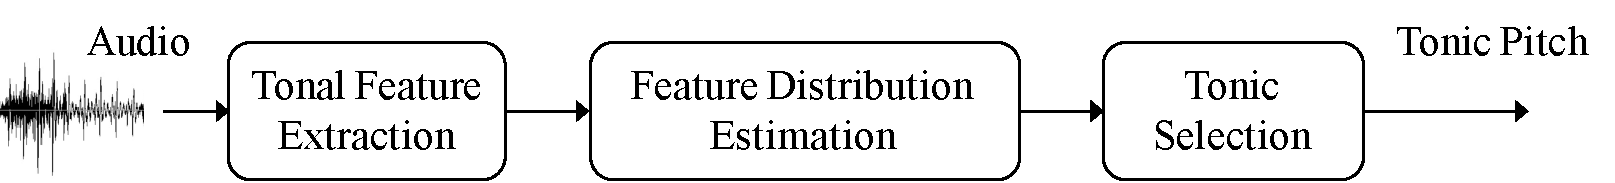
\includegraphics[width=\figSizeNinetyFive]{ch02_background/figures/tonic_identification_block_diagram.pdf}
	\end{center}
	\caption[General block diagram of tonic identification approaches]{General block diagram of the processing steps used by tonic identification approaches.}
	\label{fig:tonic_identification_general_block_diagram}
\end{figure}

In all the aforementioned approaches, the three main processing blocks are the following; feature extraction, feature distribution estimation and tonic selection. Since the task of tonic identification involves an analysis of the tonal content of the audio signal, the features extracted in the first block are always pitch related. In the second block, an estimate of the distribution of these features is obtained using either Parzen window based density estimation or by constructing a histogram. The feature distribution is then used in the third block to identify the tonic. The peaks of the distribution correspond to the most salient pitch values used in the performance (usually the \glspl{svara} of the \gls{raga}), one of which corresponds to the tonic pitch. As the most salient peak in the distribution is not guaranteed to be the tonic, various techniques are applied to select the peak that corresponds to the tonic.



\begin{sidewaystable}
	\begin{threeparttable} 
		\ra{1.1}
%		\small
		\begin{centering}
			\begin{tabular}{l L{4.5cm} L{4.5cm} L{3.5cm} }
				\tabletop			
				Method 	&	Features	&	Feature Distribution	&	Tonic Selection \\
				\tablemid			
				\acrshort{tonicid_sengupta} \citep{Sengupta2005b}	&	Pitch \citep{AKDatta_1996} & NA & Error minimization\\
				
				\acrshort{tonicid_ranjani_1}/\acrshort{tonicid_ranjani_2} \citep{ranjani2011carnatic}	&	Pitch \citep{BoersmaPaul2001} & Parzen-window-based \acrshort{pde}  & \acrshort{gmm} fitting\\
				
				\acrshort{tonicid_justin} \citep{salamon2012multipitch} & Multi-pitch salience \citep{Salamon2011} & Multi-pitch histogram & Decision tree\\
				
				\acrshort{tonicid_sankalp} \citep{gulati2012two}	& Multi-pitch salience  \citep{Salamon2011} & Multi-pitch histogram & Decision tree\\
				
				&	Predominant melody \citep{Salamon2012} & Pitch histogram & Decision tree\\
				
				\acrshort{tonicid_ashwin_1} \citep{bellur2012knowledge}	&	Pitch \citep{DeCheveigne2002}	&  \acrshort{gd} histogram & Highest peak\\
				
				\acrshort{tonicid_ashwin_2} \citep{bellur2012knowledge}	&	Pitch \citep{DeCheveigne2002}	& 	GD histogram	&
				Template matching\\
				
				\acrshort{tonicid_ashwin_2} \citep{bellur2012knowledge}	&	Pitch \citep{DeCheveigne2002}	& 	GD histogram
				& Highest peak\\
				
				\acrshort{tonicid_chordia} \citep{chordia2013joint}	& 	& 	& \\			
				
				\tablebot		
			\end{tabular}
			\par \end{centering}		
		\begin{tablenotes}
			\small
			\item[] ABBREVIATIONS: NA=Not applicable; GD=Group Delay, PDE=Probability Density Estimate
		\end{tablenotes}
			\caption[Summary of existing tonic identification approaches.]{Summary of existing tonic identification approaches.}
			\label{tab:pre_processing_tonic_identification_summary_methods}
	\end{threeparttable}
\end{sidewaystable}

In \tabref{tab:pre_processing_tonic_identification_summary_methods} we provide a summary of the existing methods for tonic identification. The common processing blocks and the main differences between them become evident from this table. A detailed review of these methods is done in~\cite{Gulati2014Tonic}. For a more detailed description of these methods we refer to their respective publications listed in Table \tabref{tab:pre_processing_tonic_identification_summary_methods}. We now discuss each of these methods within each processing block.


\subsubsection{Tonal Feature Extraction}
\label{Feature Extraction}

In the tonal feature extraction block (\figref{fig:tonic_identification_general_block_diagram}), the algorithms extract pitch-related
features from the audio signal for further processing. With the exception of \cite{salamon2012multipitch,gulati2012two}, all approaches use a single feature, the predominant pitch in the audio. Note that whilst pitch and fundamental frequency ($f_0$) are not the same (the former being a perceptual phenomenon and the latter a physical quantity), for the purpose of tonic identification the $f_0$ is considered a reliable representation of pitch. Unlike these approaches, \cite{salamon2012multipitch} uses a multi-pitch salience feature in order to exploit the tonal information provided by the drone instrument. Finally, \cite{gulati2012two} uses both the multi-pitch salience feature and the predominant melody. 

We now provide an overview of the algorithms used by the different approaches mentioned above for extracting $f_0$ and multi-pitch salience from audio recordings. \cite{ranjani2011carnatic} use the Praat software\footnote{Version 5.3.}~\cite{BoersmaPaul2001} to obtain the pitch contours. The software implements the algorithm by~\cite{boersma1993accurate}, which is primarily proposed for speech signals and has also been used for monophonic music recordings in the past. \cite{Ashwin_Istanbul2012} uses YIN, an \gls{amdf} based pitch estimation algorithm proposed by~\cite{DeCheveigne2002}. YIN is mainly developed for speech signals. As~\cite{DeCheveigne2002} make a remark,  the algorithm is informally tested on music and yet to be evaluated on polyphonic music. However, YIN has been used in a number of studies in \gls{mir} for pitch estimation from polyphonic music signals. \cite{Sengupta2005b} use a method based on \gls{psa} proposed by~\cite{AKDatta_1996} for extracting the $f_0$. Subsequently, a steady state detection is applied to the pitch contours in order to consider only the steady note regions for the analysis. Only segments of the pitch contour with a steady-state duration of at least 60 ms are used. It should be noted that this study was carried out using solo vocal performances (monophonic audio), which were carefully recorded in a studio without any kind of accompaniment present in the audio.

One of the possible caveats of the aforementioned pitch (strictly speaking, $f_0$) estimation methods is that they are all primarily designed for monophonic signals containing a single sound source. This means that the number of estimation errors could increase as we add more instruments into the mixture. While due to the heterophonic nature of \gls{iam} and the prominent lead voice monophonic pitch trackers often manage to detect the $f_0$ of the lead artist even in the presence of accompaniment instruments. One way of overcoming this problem is by using a predominant pitch estimation algorithm. \cite{gulati2012two} use the method proposed by~\cite{Salamon2012} for estimating the pitch sequence of the predominant melody from the audio signal. \cite{gulati2012two} exploit the pitch information of the melody in the second stage of their approach to identify the specific octave of the tonic pitch (the tonic pitch-class is identified during the first stage of the algorithm).

As noted earlier, some proposed methods for tonic identification~\citep{salamon2012multipitch,gulati2012two} use a multi-pitch approach. Instead of extracting the predominant melodic component from the audio signal, the methods compute a multi-pitch time-frequency representation of pitch salience over time~\citep{Salamon2011}. The motivation for using multi-pitch analysis is twofold: first, as noted earlier, the music material under investigation is non-monophonic (includes many instruments playing simultaneously). Second, the tonic is continuously reinforced by the drone instrument, and this important cue can not be exploited by only extracting a single pitch value for each frame of the audio recording. To illustrate this point, in~\figref{fig:2HarmonicSeries} we display the spectrogram of a short audio excerpt of Hindustani music. Two types of harmonic series are clearly visible in the plot: the first consists of nearly straight lines and corresponds to the drone instrument (playing Sa and Pa). The second harmonic series (which start approximately at time 1 s) corresponds to the voice of the lead performer. Since the drone instrument is constantly present in the signal, a histogram of the peaks of the salience function will have prominent peaks at the pitches of the drone instrument, and this is exploited by \cite{salamon2012multipitch,gulati2012two} for identifying the tonic. The main difference between the two approaches is that whilst~\citep{salamon2012multipitch} directly identifies the tonic pitch from the histogram, \cite{gulati2012two} divides the task into two stages: first the tonic pitch-class is identified using an extension of \cite{salamon2012multipitch}, and then the correct tonic octave is identified using the predominant melody information (see~\cite{Gulati2014Tonic} for further details).

\begin{figure}
	\begin{center}
		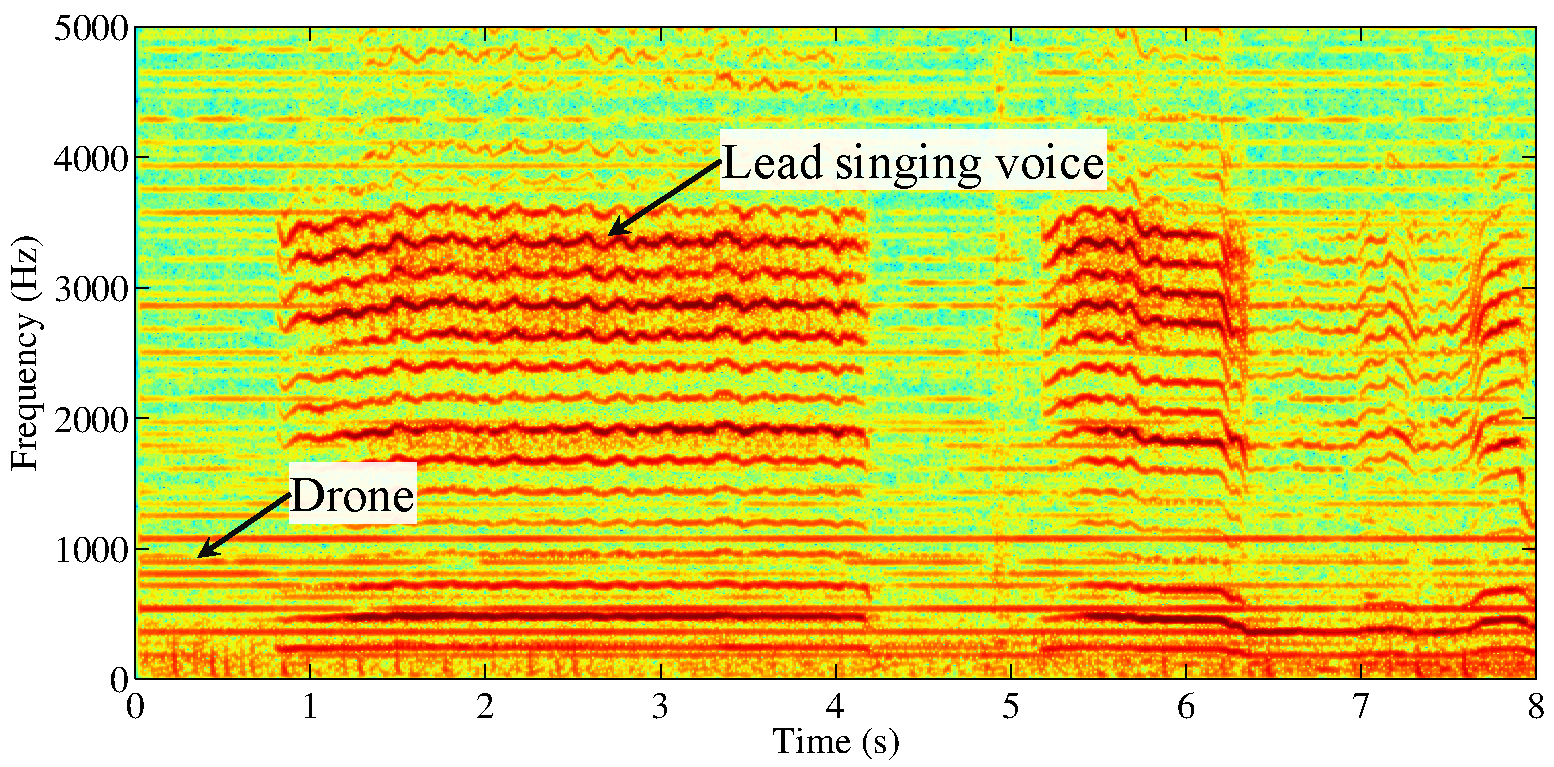
\includegraphics[width=\figSizeNinety]{ch02_background/figures/2HarmonicSeries.pdf}
	\end{center}
	\caption[Spectogram of an excerpt of Hindustani music][Spectrogram of an excerpt of Hindustani music illustrating presence of the lead voice and the drone]{Spectrogram of an excerpt of Hindustani music with two clearly visible types of harmonic series, one belonging to the drone and the other to the lead voice.}
	\label{fig:2HarmonicSeries}
\end{figure}


\subsubsection{Feature Distribution Estimation}
\label{sec:background_tonic_feature_distribution_estimation}

The tonal features extracted by the different tonic identification approaches are subsequently analyzed in a cumulative manner (cf.~block two in~\figref{fig:tonic_identification_general_block_diagram}). The pitch values from all analysis frames (whether a single value is computed per frame or multiple values) are aggregated into a pitch distribution function, which reflects the (possibly weighted) rate of occurrence of different pitch values in the entire audio excerpt. The peaks of the pitch distribution function represent the most frequent (or salient if weighting is used) pitches in the recording, one of which will be the tonic. The only exception is the approach proposed by~\cite{Sengupta2005b}, which instead of analyzing the distribution of the features, computes an aggregate error function in order to select the tonic. The methods used by the different tonic identification approaches for estimating the pitch distribution function are described below.

In~\cite{salamon2012multipitch,gulati2012two}, the pitch values of the peaks of the salience function in every frame are aggregated into a histogram. The top 10 peaks in every frame are used, in this way ensuring that in addition to the lead instrument/voice, the pitch content of other accompanying instruments is also captured, most importantly the notes played by the drone instrument. The frequency range considered for selecting the peaks of the salience function for constructing the histogram is restricted to 100-370\,Hz (note that the typical frequency range for the tonic 100-260\,Hz). The reason for computing the histogram beyond 260\,Hz even though the tonic rarely goes above this frequency is that in some cases the aforementioned methods can exploit the presence of a peak corresponding to the fifth/fourth (Pa/Ma) above the tonic in order identify the tonic pitch. Since in many cases the lead voice/instrument is considerably louder than the drone sound, the weights of the salience peaks are ignored when computing the histogram, meaning only the rate of occurrence is taken into account. As noted earlier, the result is that the pitches produced by the drone instrument (the tonic and Pa, Ma or \gls{ni}) manifest in the form of high peaks in the histogram, since the drone sounds continually in the recording. The resulting pitch distribution thus depends heavily on the notes of the drone instrument. This would not be the case if we they considered the predominant melody for computing the histogram, in which case the pitch distribution would depend on the chosen \gls{raga}, thus increasing the complexity of identifying the tonic.

\begin{figure}
	\begin{center}
		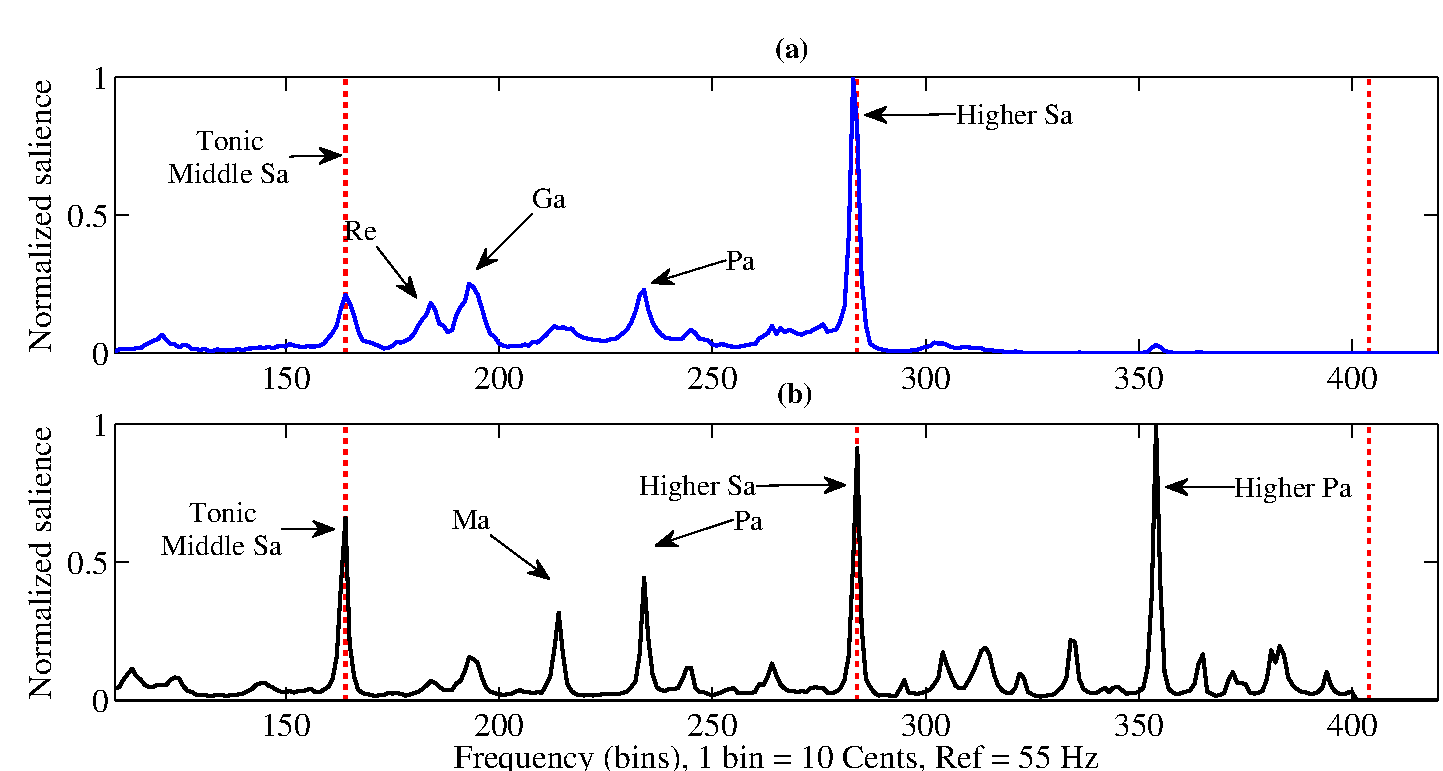
\includegraphics[width=\figSizeHundred]{ch02_background/figures/Histogram_Melody_Multipitch.pdf}
	\end{center}
	\caption[Pitch histograms constructed using two different methods]{Pitch histograms for the same excerpt constructed using (a) predominant melody (in blue) and (b) peaks of a multi-pitch salience function (in black). The tonic pitch-class locations are indicated with red dotted lines.}
	\label{fig:background_pitch_histograms_multipitch}
\end{figure}

In~\figref{fig:background_pitch_histograms_multipitch} we display two pitch histograms, computed using (a) the pitch of the predominant melody and (b) the peaks of a multi-pitch salience function. Both histograms are computed from the same three-minute audio excerpt. We see that in the histogram computed using the predominant melody (a), the prominent peaks correspond to \glspl{svara} Sa, Ga and Re (the prominent \glspl{svara} of \gls{raga} \textit{Sindh Bhairav\={\i}} ), whereas in the multi-pitch histogram (b), the top three peaks correspond to Sa (in two octaves) and Pa, which are the prominent \glspl{svara} produced by the drone instrument. 

In~\cite{Ashwin_Istanbul2012}, a histogram is constructed using a frequency range of 40-800\,Hz with a 1\,Hz resolution and later post processed using a \gls{gd} function. The authors show that by assuming that the constructed pitch histogram is the squared magnitude of resonators in parallel, group delay functions can be applied to obtain a better resolution for the peaks in the resulting histogram. It is also shown that a group delay function accentuates peaks with lesser bandwidths. Given that the \gls{shadja} (tonic pitch-class) and \gls{panchama} (fifth of the tonic pitch-class) in all octaves are relatively less inflected, this characteristic of the \gls{gd} function is shown to be beneficial for improving the accuracy of tonic identification. The processed histograms are referred to as \gls{gd} histograms.

\cite{Ashwin_Istanbul2012} also propose the concept of segmented histograms. In order to exploit the omnipresence of the \gls{shadja},  it is proposed that, given the pitch contour for an item of music, the contour is segmented into smaller units and a \gls{gd} histogram is constructed for each of these smaller units. Given that \gls{shadja} will be present in all the units, the peak corresponding to the \gls{shadja} will be enhanced in the corresponding \gls{gd} histograms. The individual histograms are then multiplied bin-wise. This also helps in reducing the height of the non \gls{shadja} peaks which might not be present in all the segments. Tonic selection is then performed on the resulting histogram, referred to as the segmented \gls{gd} histogram.

Instead of using a histogram, \cite{ranjani2011carnatic} use a Parzen window estimator to compute a pitch density function~\citep{Bishop,DudaHart2000}. Parzen window estimators (or kernel density estimators) are non-parametric density estimators. The choice of kernel function can control the smoothness of the estimated density. They are widely used as an alternative to histograms to alleviate the artificial discontinuities at the boundaries of the bins of the histogram, and aid in a smoother peak picking process. In addition, they do not require partitioning of data into distinct bins. \cite{ranjani2011carnatic} use parzen window estimators with Gaussian kernels for estimating the density of the extracted pitch frequencies.


\subsubsection{Tonic selection}
\label{sec:tonic_selection}

In the previous section we discussed different ways to compute the pitch distribution function. This section presents the last processing block shown in~\figref{fig:tonic_identification_general_block_diagram}, where the pitch distribution function is used to identify the tonic pitch. The peaks of the pitch distribution function correspond to the most frequent (or salient) pitches present in the audio signal. Depending on how the pitch distribution is computed the peaks will coincide with the \glspl{svara} of the \gls{raga} used in the rendition or with the \glspl{svara} produced by the drone instrument. The problem of tonic identification is thus reduced to selecting the peak of the distribution that corresponds to the tonic of the lead artist. As noted earlier, the peak corresponding to the tonic pitch is not always the highest peak in the distribution. For this reason, various strategies are have been proposed for analyzing the pitch distribution and selecting the peak that corresponds to the tonic. The complexity of the approaches varies from simply selecting the highest peak of the histogram to the application of machine learning algorithms in order to automatically learn the best set of rules for selecting the tonic peak. The different tonic selection strategies used in the literature are presented below.

\cite{ranjani2011carnatic} model the pitch distribution using semi-continuous Gaussian mixtures~\cite{Huang2001}, motivated by the following two musical cues in Indian art music; first, the relative positions of the \glspl{svara} with respect to the tonic hover around a mean ratio~\citep{Krishnaswamy2003} and second, the \gls{shadja} (tonic pitch-class) and \gls{panchama} (fifth of the tonic pitch-class) are the prakrthi \glspl{svara} which means they are sung/played without any inflections~\citep{Manikandan2004,Krishnaswamyicassp2003}. Peaks of the pitch density function within a suitable pitch range are selected as possible tonic candidates. The variance of the pitch distribution around the peaks is estimated by modeling each tonic candidate (i.e.~peak) with a Gaussian distribution. As noted above, one of the key characteristics of \gls{shadja} and \gls{panchama} is that they do not vary (in pitch) throughout the performance. Thus, the parameters of the Gaussian model are used to infer the correct tonic candidate. The pitch range used for selecting tonic candidates is 100-250\,Hz. When the editorial metadata of the audio recording is known, the pitch range is further constrained depending on the gender of the lead artist. The range for male singers is set to 100-195\,Hz and for female singers is set to 135-250\,Hz.

\cite{salamon2012multipitch,gulati2012two} use a classification based approach to identify the peak of the multi-pitch histogram that corresponds to the tonic pitch~\citep{salamon2012multipitch} or tonic pitch-class~\citep{gulati2012two}. Since all the pitches in a performance are in relation to the tonic, the relationships between the peaks of the histogram (height and distance) are used to compute a set of features, which are then used to train a classifier for identifying which peak corresponds to the tonic. In this way, rather than having to manually define a template for selecting the tonic, an optimal set of rules are learned automatically using machine learning. The authors extract height and distance related features for the top 10 peaks in the multi-pitch histogram. The authors show that for the tonic identification task the C4.5 decision tree classifier~\citep{Quinlan:1993:CPM:152181} yields the highest classification accuracy. 

\cite{gulati2012two} uses a similar classification-based approach to first identify the peak of the histogram that corresponds to the tonic pitch-class. The correct tonic octave is then determined in the second stage of processing, which is also classification-based. For every candidate tonic pitch (candidates have the same pitch class but are in different octaves) a set of 25 features is computed. The features are the values of the melody histogram at 25 equally spaced locations spanning two octaves centered around the tonic pitch candidate. The classification is a two-class problem: either the pitch candidate is in the correct octave, or it is not. As done in~\cite{salamon2012multipitch}, a C4.5 decision tree is trained using the Weka data-mining software for the classification. For a detailed description of the method we refer to~\cite{SGulati_MThesis2012}.

\cite{Sengupta2005b} use an error minimization technique to identify the tonic. This is a brute force approach in which a large number of pitch values within a pre-defined frequency range are considered as candidates for the tonic pitch. A cumulative deviation is computed between the steady state regions of the pitch contour (described in~\secref{sec:background_tonic_feature_distribution_estimation}) and the pitch values of the closest notes to these regions, which are obtained using three different tuning schemas given a tonic candidate. The tonic candidate which results in the minimum deviation is selected as the tonic of the musical excerpt.

\cite{Ashwin_Istanbul2012} propose a simple approach, picking the highest peak of the pitch distribution as the tonic. In two out of the three proposed variants of their method, the bin value of the highest peak of the segmented \gls{gd} pitch histogram is selected as the tonic pitch. The frequency range of the histogram is restricted to 100-250\,Hz. When the gender information of the lead artist for an audio recording is available, this range is further restricted. In addition to the simple highest peak approach, \cite{Ashwin_Istanbul2012} also propose a template matching process to identify tonic. This procedure is comparable to the Semi-continuous GMM fitting proposed by~\citep{ranjani2011carnatic}, which exploits the smaller degree of pitch variation around \gls{shadja} and \gls{panchama}. The template that the authors use to identify the tonic candidate uses three octaves and consider the pitch distribution values at tonic and its fifth (Pa) in different octaves. For more information we refer to~\cite{Gulati2014Tonic}.


As we see from this review on the task of tonic identification, a variety of methods are proposed in the literature. These methods vary considerable within each processing block of the task. Many of these studies show promising results. However, since they are evaluated on different datasets with different sets of measures and evaluation setup, they cannot be directly compared.  We note that in none of these studies an attempt is made to compare the performance with other studies. In order to deeply understand the strengths and shortcomings of these approaches on different types of music material it is essential that they are compared under the same experimental setup and using the same music collection. 


\subsection{Melodic Pattern Processing}
\label{sec:sota_pattern_processing_iam}

\COMMENT{Images for Phrases, highlighting transients and their importance}

\begin{sidewaystable}
	\begin{threeparttable} 
%		\setlength{\tabcolsep}{2pt}
		\small
		\ra{1.2}
		\begin{centering}
			\begin{tabular}{l L{1.5cm} L{2.5cm} L{2cm} L{2cm} L{1.5cm} L{1.5cm} L{.5cm} L{.5cm} L{0.6cm} L{0.6cm} L{0.6cm}}
\tabletop
			Method	& Task & Melody Representation & Segmentation & Similarity Measure & Speed-up & \#\Glspl{raga} & \#Rec & \#Patt & \#Occ \tabularnewline
\tablemid
				\cite{ishwar2012motivic} & Distinction & Continuous & GT annotations & \acrshort{hmm} & - & 5\tnote{c} & NA & 6 & 431\tabularnewline
				\cite{Ross2012} & Detection & Continous & Pa \gls{nyas} & \acrshort{dtw} & Segmentation & 1\tnote{h} & 2 & 2 & 107\tabularnewline
				\cite{Ross2012b} & Detection & Continous, SAX-12,1200 & Sama location & Euc., \acrshort{dtw} & Segmentaion & 3\tnote{h} & 4 & 3 & 107\tabularnewline
				\cite{Ishwar2013} & Detection & Stationary point, Continuous & Bruteforce & \acrshort{rlcs} & Two pass method & 2\tnote{c} & 47 & 4 & 173\tabularnewline
				\cite{rao2013distinguishing} & Distinction & Continuous & GT annotations & \acrshort{dtw} & - & 1\tnote{h} & 8 & 3 & 268\tabularnewline
				\cite{Dutta2014} & Discovery & Stationary point,  Continuous & Bruteforce & \acrshort{rlcs} & - & 5\tnote{c} & NA & - & -\tabularnewline
				\cite{dutta2014modified} & Detection & Stationary point, Continuous & NA & Modified-\acrshort{rlcs} & Two pass method & 1\tnote{c} & 16 & NA & 59\tabularnewline
				\multirow{2}{*}{\cite{Rao2014}} & Distinction & Continous & GT annotations & \acrshort{dtw} & - & 1\tnote{h} & 8 & 3 & 268\tabularnewline
				& Distinction & Continous & GT annotations & \acrshort{hmm} & - & 5\tnote{c} & NA & 10 & 652\tabularnewline
				\cite{ganguli2015efficient} & Detection & \acrshort{bss}, Transcription & Implicit & Smith-Waterman & Discretization & 34\tnote{h} & 50 & NA & 1075\tabularnewline
\tablebot			

			\end{tabular}
			\par \end{centering}
		
		\begin{tablenotes}
			\small
			\item[h] Hindustani music collection
			\item[c] Carnatic music collection
			\vspace{0.20cm} \\
			\item[] ABBREVIATIONS: \#Rec=Number of recordings;       \#Patt=Number of unique patterns; \#Occ=Total number of annotated occurrences of the patterns; GT=Ground truth; NA=Not available; ``-''= Not applicable; Euc.=Euclidean distance.
						
		\end{tablenotes}
		\caption[Summary of the melodic pattern processing methods for \gls{iam}]{Summary of the methods proposed in the literature for melodic pattern processing in \gls{iam}. \COMMENT{Confirm with vignesh the number of phrases in his study, 2 or 4. Format the table}}
		\label{tab:pattern_processing_iam}
	\end{threeparttable}
\end{sidewaystable}

In this section we review the existing approaches for melodic pattern processing in audio collections of \gls{iam}. By melodic pattern processing we jointly refer to a number of research tasks that involve computational analysis of melodic patterns such as pattern similarity, pattern detection and pattern discovery. Analysis of melodic patterns is a well established research task in \gls{mir}~(\secref{sec:pattern_processin_in_music}). However, for \gls{iam}, despite the importance of melodic patterns in the \gls{raga} framework this computational task has gained attention only recently, mainly during the course of this dissertation. 

In~\tabref{tab:pattern_processing_iam} we summarize the existing approaches for pattern processing in \gls{iam} and provide relevant details to better compare these approaches and get an overall perspective. We see that there are three closely related but different pattern processing tasks that these approaches address (\tabref{tab:pattern_processing_iam}); 1) Pattern detection, where given a query melodic pattern the objective is to retrieve its other occurrences in the test audio recordings~\citep{Ross2012,Ross2012b,Ishwar2013,dutta2014modified,ganguli2015efficient}, 2) Pattern distinction, where given a query pattern the objective is to retrieve its other instances from a pool of annotated melodic patterns~\citep{ishwar2012motivic,rao2013distinguishing,Rao2014}, 3) Pattern discovery, where given a collection of music recordings the objective is to discover melodic patterns in the absence of any ground truth annotations of the melodic patterns~\citep{Dutta2014}. The task of pattern distinction can be considered as a subtask of pattern detection, with the main differences being the absence of the irrelevant patterns in the search space and the use of pre-segmented melodic patterns. We differentiate between these two tasks in this review because the complexity involved in these tasks are considerably different. Also, the approaches proposed for pattern distinction do not address the issues related with the computational complexity, a challenge often encountered in the task of pattern detection and discovery. Note that there are a few studies done on detection and modeling of specific melodic ornaments in Hindustani and Carnatic music~\citep{Subramanian2012,Datta2007,narayan2014detection,pratyush_2010}. We do not consider these studies in the current review since they focus on a particular type of short-duration melodic ornament (or gesture). Moreover, the methodology used in some of these approaches is already covered in our review of the other methods.


As seen from~\tabref{tab:pattern_processing_iam}, a majority of the existing approaches follow a supervised approach and focus on the task of pattern detection or pattern distinction. This can be attributed to the challenges involved in the task of pattern discovery, specifically in terms of the computational complexity. In addition, since this research topic has recently gained attention in \gls{mir} for \gls{iam}, the primary focus of the approaches in the beginning is to devise meaningful melodic similarity model. Based on the description of these approaches there are three main processing units involved in this task; melody representation, melody segmentation and similarity (or dissimilarity) computation. There is often an interplay between the choices made within these three units, specifically between the melody representation and the similarity measure. As it is also highlighted in~\cite{gomez2003melody}, pitch and timing variations across occurrences of the melodic patterns can be either handled in the melody representation or during the computation of the melodic similarity. In the former case, a generic or a musically agnostic distance measure might be sufficient for computing melodic similarity. Whereas, in the latter, a music specific distance measure that can incorporate domain knowledge and can handle timing and pitch variations is required. 

We first review the existing approaches in terms of the three processing units mentioned above. From~\tabref{tab:pattern_processing_iam} we notice that with only a couple of exceptions~\citep{Ross2012b,ganguli2015efficient} all other approaches work with a fine grained continuous melody representation. This to a large extent is attributed to the characteristics of the melodies in \gls{iam} due to which the extraction of a reliable symbolic or discrete melody representation becomes a challenging task~\citep{widdess1994involving}. Moreover, the transitory melodic regions between the \glspl{svara} in a melody are found to be important in the computation of melodic similarity~\citep{Datta2007,gupta2012objective}, which are lost in a simple transcription of melodies. \cite{Ross2012b,ganguli2015efficient} examine the affect of abstracting the melody representation by using techniques such as \gls{sax}~\citep{Lin2003} and \gls{bss}~\citep{tanaka2005discovery}. \cite{ganguli2015efficient} also propose a heuristic-based pseudo melody transcription approach to obtain a discrete melody representation. It was found that though these representations reduce the computational cost by a significant factor. However, the accuracy remains inferior compared to the continuous melody representation (considering the best performing distance measure for both the types of melody representations)~\cite{Ross2012b,ganguli2015efficient}. Moreover, these discrete representations are evaluated on a small dataset comprising a specific style of singing within Hindustani music. Therefore, applicability of such abstracted melody representations to all types of melodic styles in both Hindustani and Carnatic music is questionable. \cite{Ishwar2013,Dutta2014,dutta2014modified} propose an abstracted melodic representation that exploits specific melodic characteristics of Carnatic music. To represent a melody the authors consider only the stationary points (where the slope becomes zero) in the continuous melody representation. However, such a representation is too coarse to compute a reliable melodic similarity, and therefore, it is primarily used to prune the search space in order to reduce the computational cost. The final computation is done by using a continuous melody representation. Overall, we see that devising an abstracted melody representation that can encapsulate and abstract both the timing and the pitch variations is a challenging task for melodies in \gls{iam}. We also notice that a continuous melody representation appears to be the most versatile representation as it places minimal assumptions on the melodic style. 

As noted before, an important aspect in pattern detection is melody segmentation. While there are well studied models for melody segmentation in symbolic representation of Western classical music~\citep{Cambouropoulos2006,rodriguez2014comparing}, to the best of our knowledge such segmentation models for \gls{iam} in audio recordings are inexistent. As a result of which, approaches for pattern detection in \gls{iam} either tend to use a brute force segmentation strategy or use a local alignment-based distance measure that does not require an explicit melody segmentation~(\tabref{tab:pattern_processing_iam}). \cite{Ross2012,Ross2012b} detect specific rhythmic and melodic landmarks (\gls{sama} locations and \gls{nyas} \gls{svara} onsets) in the audio recordings to determine the location of the potential melodic pattern candidates. However, these approaches are too specific to a certain type of melodic patterns, musical style and to only slow tempo (vilambit laya) music compositions. For example, \gls{sama} location can indicate roughly the onset of a \gls{mukhda} phrase in an recording of Hindustani music. But, it has no musically established relationship with the location of the characteristic melodic phrases of \glspl{raga}. Similarly, the Pa \gls{nyas} segmentation strategy followed in~\cite{Ross2012} can work only with the melodic phrases ending in the Pa \gls{svara}, and mainly for slow tempo compositions where the concept of \gls{nyas} \gls{svara} is evident. Thus, these approaches do not generalize and scale to other types of melodic patterns and to large music collections. Moreover, detecting these landmarks in itself is a challenging task~\citep{srinivasamurthy2014supervised,gulati2014Landmark}. Overall, we see that there is a lack of phrase-level segmentation models for melodies in \gls{iam}.

Melodic similarity (or dissimilarity) measure is another crucial block in the melodic pattern processing tasks. From \tabref{tab:pattern_processing_iam} we see that a majority of the approaches use a dynamic programming-based similarity measure. \cite{Ross2012,Ross2012b,rao2013distinguishing,Rao2014} use a similarity measure based on different variants \gls{dtw}, \cite{Ishwar2013,Dutta2014,dutta2014modified} use a \gls{rlcs}-based similarity measure, and \cite{ganguli2015efficient} employ Smith-Waterman algorithm~\citep{smith1981identification} to compute melodic similarity. The dominance of dynamic programming-based similarity measures can be attributed to the fact that the melodic patterns in \gls{iam} undergo a large degree of non-linear timing variations, which can further be attributed to the improvisatory nature of this music tradition. Computing sequence similarity without any temporal alignment such as in Euclidean distance falls short of measuring a meaningful melodic similarity in \gls{iam}~\citep{Ross2012b}. Although a thorough comparison of the Euclidean distance with the dynamic programming-based similarity measures for the same melody representation is lacking in the literature. Some of the existing studies also propose enhancements to the well-known distance measures. \cite{dutta2014modified} propose to modify the intermediate steps involved in the computation of the \gls{rlcs} distance to make it more suitable to melodic sequences. These modifications are reported to result in an improvement in the precision of the system, while maintaining the same recall. However, the study is conducted using only 59 pattern instances in 16 excerpts belonging to only one \gls{raga}. \cite{Rao2014} propose to learn an optimal shape of the global path constrained applied in the \gls{dtw}-based distance measure. However, the learned global constraint degraded the performance of the method. Moreover, since the constraint learning is performed for a particular pattern category, such a technique is not applicable to an unseen data as is the case in the task of pattern discovery. In contrast to these time-series matching-based approaches, there are a few approaches that use statistical pattern matching paradigms. \cite{ishwar2012motivic,Rao2014} consider this task similar to that of a keyword spotting in speech, and therefore utilize \glspl{hmm} to essentially perform pattern classification. The evaluations of the \gls{hmm}-based system show promising results. However, the authors address a relatively easier task of pattern distinction, where the search space did not contain any irrelevant pattern candidates. Moreover, since there was no baseline system considered in the evaluations, a comparison of the \gls{hmm}-based approach to the other methods is subjected to a comparative evaluation.

We now compare the existing approaches in terms of the other relevant aspects involved in the task of melodic pattern processing. An important consideration in the pattern detection and discovery task for sizable datasets is the computational complexity. Since the similarity measures that perform well as noted above are mainly based on dynamic programming, computational complexity becomes even a bigger concern. As seen from~\tabref{tab:pattern_processing_iam} not every approach addresses this issue. This can be due to the small size of the datasets used to evaluate the approaches, for which these systems are not computationally intractable. \cite{ganguli2015efficient} improve the computational efficiency of their method by using an abstracted low-dimensional discrete melody representation. However, as seen before, the performance of such a system is inferior to that using a continuous melody representation, and the scalability of such an approach to diverse music material is questionable. Furthermore, the accuracy of such an approach is always limited by the performance of the melody transcription system. Another type of optimization is to perform the task of pattern detection in two stages as proposed by~\cite{dutta2014modified,Ishwar2013}. In the first stage a coarse melody representation can be used to identify the regions in the audio recordings that are more likely to contain the relevant pattern. Such a coarse melody representation drastically reduces the computational cost involved in the operation. Once the search spaced is pruned, in the second stage, a fine grained continuous melody representation can be used to reliably detect the pattern occurrences. The coarse melody representation proposed by~\cite{Ishwar2013} is specific to Carnatic music, and is not generalizable to Hindustani music. Besides, this method does not compute a theoretical lower-bound, and the pruning is based on an empirically determined threshold. This means that it is not very suitable for tasks such as pattern discovery, where determining a musically relevant similarity threshold in itself is a challenge. Furthermore, the first stage of this method does not result in a perfect (100\%) recall, and therefore, it can potentially become a bottleneck for the system. Some other proposals for reducing the computational complexity involve top-down segmentation methods that exploit the specific type of melodic and rhythmic landmarks such as \gls{sama} and \gls{nyas} onsets~\citep{Ross2012,Ross2012b}. Occurrences of a certain types of melodic phrases are marked by these events. However, as explained earlier, such an approach makes the system tuned to a particular type of melodic patterns and musical forms within Hindustani music. Overall, we notice that the existing approaches do not utilize any generalizable algorithms to reduce the computational complexity of the task. 

There are several venues for improvement in the existing approaches, one of which is the evaluation setup. Apart from the fact that the evaluation setup is considerably different across studies, even within a study it needs to improve to generate reliable results. Most of the approaches are evaluated with only a few recordings belonging to a handful of \glspl{raga}. Thus, dataset size and diversity is one of the major limitations of the experimental setup used in the existing studies. The evaluation measures used by a number of these approaches are ad-hoc. For example, \cite{ganguli2015efficient} uses only first five phrases taken from the starting of the recordings to evaluate the system. Even though the other annotated pattern instances when retrieved are regarded as true hits. Thus, not considering all the annotated pattern instances as a query creates an evaluation bias. Another example is in~\cite{Ishwar2013}, where the authors measure precision, recall and F-measure using only the top ten retrieved results, wherein the number of relevant patterns in the system are of the order of 100. Also, the procedure followed to calculate these measures in such a specific scenario is not described in the article. Thus, there is a need to promote and use well established evaluation metrics typically used in information retrieval tasks to make the results more comparable. 

An observation that can be made from~\tabref{tab:pattern_processing_iam} is that none of the existing approaches perform evaluation using both Hindustani and Carnatic music collections. The melodic characteristics between these two music traditions vary considerably. Thus, evaluating the same system with both the music traditions can provide new insights in to the shortcomings and strengths of the different melodic representations and similarity measures. Another observation is that there is only one method that addresses the task of pattern discovery~\cite{Dutta2014}. The proposed method is shown to work with short duration (~15\,seconds) audio excerpts comprising the first line of the compositions, which are specifically recorded and segmented for the study. Scalability of such an approach to hundreds of hours of music collections is questionable. Understandably, pattern discovery is a complex and a computationally expensive task compared to pattern detection. Nonetheless, there should be more research efforts directed towards it, especially since the size of the datasets used in the supervised approaches tends to be small owing to the challenges involved in the annotation process.
\COMMENT{Rephrasing}

Based on our discussion above, we see that there are a variety of approaches proposed for melodic pattern processing in \gls{iam}. However, a direct comparison across these approaches cannot be made, since these approaches are evaluated on different experimental setup. A systematic improvement in these approaches calls for a comprehensive comparative evaluation to understand their limitation and strengths on different type of music content within \gls{iam}. Apart from comparing the existing approaches directly, there are several other aspects that require a systematic evaluation. For example, an optimal sampling rate is an important consideration in a continuous melody representation. But, despite the fact that most of the approaches use such a representation, they do not study this aspect. Similarly, none of the approaches except~\cite{Rao2014} address the issue of pitch octave transposition, which is frequently encountered across repeated instances of melodic patterns. Other issues regarding the redundancy filtering and the characterization of the discovered melodic patterns are also to be addressed. Thus, we see that there is a large scope of improvement in the existing approaches and there are a number of novel research issues to be addressed. \COMMENT{Rephrasing}


\subsection{\Glsentrytext{raga} Recognition}
\label{sec:sota_raga_recognition}

\COMMENT{Images for pitch distributions}

\begin{sidewaystable}
	\begin{threeparttable} 
		\ra{1.4}
%		\setlength{\tabcolsep}{1pt}
		\small
		\begin{centering}
			\begin{tabular}{l L{1.85cm} L{1.85cm} L{1.85cm} L{2cm} L{1.5cm} L{2cm} L{2cm}}
				\tabletop
				Methods & \Gls{svara} set & \Gls{svara} salience & \Gls{svara} intonation & \gls{arohana}-\gls{avrohana} & Melodic phrases & \Gls{svara} discretization & Temporal aspects\tabularnewline
				\tablemid
				\cite{pandey2003tansen} &  &  &  & $\bullet$ & $\bullet$ & Yes & $\bullet$\tabularnewline
				\cite{chordia2007raag} & $\bullet$ & $\bullet$ &  & $\bullet$ &  & Yes & $\bullet$\tabularnewline
				\cite{belle2009raga} & $\bullet$ & $\bullet$ & $\bullet$ &  &  & No & \tabularnewline
				\cite{Shetty2009} & $\bullet$ &  &  & $\bullet$ &  & Yes & $\bullet$\tabularnewline
				\cite{sridhar2009raga} & $\bullet$ &  &  & $\bullet$ &  & Yes & $\bullet$\tabularnewline
				\cite{koduri2011survey} & $\bullet$ & $\bullet$ &  &  &  & Yes & \tabularnewline
				\cite{ranjani2011carnatic} & $\bullet$ &  &  &  &  & No & \tabularnewline
				\cite{chakraborty2012object} & $\bullet$ &  &  &  &  & Yes & \tabularnewline
				\cite{koduri2012raga} & $\bullet$ & $\bullet$ & $\bullet$ &  &  & Both & \tabularnewline
				\cite{chordia2013joint} & $\bullet$ & $\bullet$ & $\bullet$ &  &  & No & \tabularnewline
				\cite{dighe2013scale} & $\bullet$ & $\bullet$ &  & $\bullet$ &  & Yes & $\bullet$\tabularnewline
				\cite{dighe2013swara} & $\bullet$ & $\bullet$ &  &  &  & Yes & \tabularnewline
				\cite{koduri2014intonation} & $\bullet$ & $\bullet$ & $\bullet$ &  &  & No & \tabularnewline
				\cite{kumar2014identifying} & $\bullet$ & $\bullet$ & $\bullet$ & $\bullet$ &  & Yes & $\bullet$\tabularnewline
				\cite{shrey_ISMIR_2015}\tnote{a} &  &  &  &  & $\bullet$ & No & $\bullet$\tabularnewline	
				\tablebot
			\end{tabular}
			\par \end{centering}
		
		\begin{tablenotes}
			\item[a] This method performs \gls{raga} verification and not recognition
		\end{tablenotes}
		\caption[Melodic characteristics utilized by the existing \gls{raga} recognition methods]{\Gls{raga} recognition methods proposed in the literature along with the melodic characteristics they utilize to perform the task. We also indicate if a method uses a discrete \gls{svara} representation of melody. The methods are arranged in the chronological order.}
		\label{tab:raga_recognition_methods_melodic_characteristics}
	\end{threeparttable}
\end{sidewaystable}


\begin{sidewaystable}
	\begin{threeparttable} 
\scriptsize
		\ra{1.1}
		\begin{centering}
			\begin{tabular}{l l P{2cm} P{3cm} P{2.5cm} L{1cm} P{1.5cm} P{2cm}}
				\hline 
				& \textbf{Tonal Feature} & \textbf{Tonic } & \textbf{Feature} & \textbf{Recognition Method} & \textbf{\#Ragas} & \textbf{Dataset (Dur./Num)}\tnote{i} & \textbf{Audio Type}\tabularnewline
				\hline 
				\cite{pandey2003tansen} & \cite{BoersmaPaul2001}\tnote{p} & Fixed frequency & Svara sequence & \acrshort{hmm} and \acrshort{ngram} & 2 & NA / 31 & Monophonic\tabularnewline
				\cite{chordia2007raag} & \cite{sun2000pitch}\tnote{p} & Manual & PCD, PCDD & \acrshort{svm} classifier & 31 & 20 / 127 & Monophonic\tabularnewline
				\cite{belle2009raga} & \cite{rao2009improving}\tnote{p} & Manual & PD (parameterized) & \acrshort{knn} classifier & 4 & 0.6 / 10 & Polyphonic\tabularnewline
				\cite{Shetty2009} & \cite{sridhar_2006_svara}\tnote{p} & Fixed frequency & \#Svaras, its combinations, Vakra svaras & Neural Network classifier & 20 & NA / 90 & Monophonic\tabularnewline
				\cite{sridhar2009raga} & \cite{lee2006automatic}\tnote{p} & Singer identification & Svara set, its sequence & String matching & 3 & NA / 30 & Polyphonic\tabularnewline
				\cite{koduri2011survey} & \cite{rao2010vocal}\tnote{p} & Brute force & PCD & \acrshort{knn} classifier & 10 & 2.82 / 170 & Polypohonic\tabularnewline
				\cite{ranjani2011carnatic} & \cite{BoersmaPaul2001}\tnote{p} & GMM fitting & PDE & SC-GMM and Set matching & 7 & NA / 48 & Polyphonic\tabularnewline
				\cite{chakraborty2012object} & \cite{sengupta1990study}\tnote{p} & Error minimization & Svara set & Set matching & NA & NA / NA & NA\tabularnewline
				\cite{koduri2012raga} & \cite{Salamon2012}\tnote{p} & Multipitch-based & PCD variants & \acrshort{knn} classifier & 43 & NA / 215 & Polyphonic\tabularnewline
				\cite{chordia2013joint} & \cite{camacho2007swipe}\tnote{p} & Brute force & PCD variants & \acrshort{knn} and statistical classifiers & 31 & 20 / 127 & Monophonic\tabularnewline
				\cite{dighe2013scale} & Chroma~\citep{lartillot2008matlab}\tnote{c} & Brute force (Vadi-based) & Chroma, Timbre features & \acrshort{hmm}  & 4 & 9.33 / 56 & Polyphonic\tabularnewline
				\cite{dighe2013swara} & \citep{lartillot2008matlab}\tnote{c} & Brute force (Vadi-based) & PCD variant & Random Forest & 8 & 16.8 / 117 & Polyphonic\tabularnewline
				\cite{koduri2014intonation} & \cite{Salamon2012}\tnote{p} & Multipitch-based & PCD (parameterized)  & Several classifiers & ?? & ?? & Polyphonic\tabularnewline
				\cite{kumar2014identifying} & \cite{Salamon2012}\tnote{p} & Brute force & PCD + \acrshort{ngram} distribution & \acrshort{svm} classifier  & 10 & 2.82 / 170 & Polyphonic\tabularnewline
				\cite{shrey_ISMIR_2015}{*} & \cite{Salamon2012}\tnote{p} & Cepstrum-based & Pitch contours & LCSS with \acrshort{knn} & 30 & 3 / 254 & Polyophonic\tabularnewline
				\hline 
			\end{tabular}
			\par \end{centering}
		\begin{tablenotes}
			\item[i] In the case of multiple datasets we list the larger one
			\item[p] Pitch extraction algorithm
			\item[c] Chroma extraction algorithm
			\item[*] This method performs \gls{raga} verification and not recognition
		\end{tablenotes}
		\caption[Summary of the existing \gls{raga} recognition methods]{Summary of the \Gls{raga} recognition methods proposed in the literature. The methods are arranged in the chronological order. \TODO{review the approaches and verify. Put specific resolution of PCD and mark if they used KDE based PCD? also make it consistent the vocabulary. Clean it further and use more meaningful descriptor names. Both Dighe paper use chroma feature...chromagram types...not PCD variant. Verify all these details..add abbreviations}}
		\label{tab:raga_recognition_methods_details}
	\end{threeparttable}
\end{sidewaystable}

Recognizing automatically the \gls{raga} of a given audio recording is one of the most important tasks in melodic description of \gls{iam}. In this section we present a review of the existing computational approaches for automatic \gls{raga} recognition in audio collections of \gls{iam}. Our main objective in this review is to consolidate existing work on automatic \gls{raga} recognition, identify the strengths and shortcomings of different methodologies, and finally, identify potential venues of improvement.

The accuracy of a \gls{raga} recognition system largely depends on the size of the dataset in terms of the number of \glspl{raga} and also on the chosen set of \glspl{raga}. The task becomes even more challenging when the chosen set of \glspl{raga} in the dataset share a common set of \glspl{svara} and are allied \glspl{raga}~(\secref{sec:allied_ragas}). Since the approaches reviewed in this section are evaluated on different datasets (typically compiled for a single study, and is not publicly made available), we refrain from comparing absolute \gls{raga} recognition accuracies across studies. 

We now proceed to review the existing \gls{raga} recognition approaches. Due to the central role of the \gls{raga} framework in \gls{iam}, its automatic identification is one of the most important research topics in computational analysis of this music tradition. Over the last couple of decades there have been several approaches proposed for this task. In \tabref{tab:raga_recognition_methods_melodic_characteristics} and \tabref{tab:raga_recognition_methods_details} we summarize the prominent existing approaches for \gls{raga} recognition. Both the tables comprise exactly the same set of approaches, but differ in terms of the type of information provided for each approach. In \tabref{tab:raga_recognition_methods_melodic_characteristics} we indicate the different characteristic features of a \gls{raga} that these approaches exploit to perform the task. The melodic attributes that we have considered in the summary are; \gls{svara} set, \gls{svara} salience, \gls{svara} intonation, \gls{arohana}-\gls{avrohana} and melodic phrases. In addition, to get a better understanding of these approaches, we also mark if an approach uses a discretized melodic representation, and if it considers the temporal aspects of the melody to perform the task. In \tabref{tab:raga_recognition_methods_details} we provide the relevant details for each approach in terms of the common processing blocks such as the feature extraction, the tonic identification, the learning method used to recognize \glspl{raga}, and the other relevant dataset details. With both these tables we get an bird's-eye view of the existing work done in \gls{raga} recognition.

From \tabref{tab:raga_recognition_methods_melodic_characteristics} we see that the most frequently used melodic attribute is the set of \glspl{svara} in a \gls{raga}, which is also computationally one of the most basic features to extract. \Gls{svara} set is considered as a feature for \gls{raga} recognition in a both explicit and implicit manner by different approaches. \citep{chakraborty2012object,ranjani2011carnatic} explicitly extract the comprising set of \glspl{svara} in an audio recording. The \gls{raga} of the recording is then identified by matching the estimated \gls{svara} set with the stored set for each \gls{raga}. The exact procedure followed to map the estimated \gls{svara} set with a unique \gls{raga} label is missing in the articles. As can be imagined, it is a rather naive approach since there are several \glspl{raga} that share the same set of \glspl{svara} and are differentiated based on more elaborate melodic and temporal characteristics.

Along with the set of \glspl{svara}, \gls{raga} grammar also defines the functional roles of these \glspl{svara}~(\secref{sec:melody_in_iam}). In particular, there is a vocabulary to describe the salience of the \glspl{svara} in a melody such as \gls{vadi} and \gls{samvadi} (the two most salient \glspl{svara} in a melody). Thus, one of the ways to differentiate between the \glspl{raga} that share a common set of \glspl{svara} is to also consider the salience of the comprising \glspl{svara} in the analysis. Computing \gls{svara} salience for all the possible \glspl{svara} frequencies implicitly incorporates the \gls{svara} set feature as well. This is the reason why this feature appears for nearly all the approaches mentioned in \tabref{tab:raga_recognition_methods_melodic_characteristics}. \cite{chordia2007raag} propose a feature that jointly incorporates the presence and the salience of different \glspl{svara} in a melody for recognizing \glspl{raga}. The authors represent \gls{svara} saliences using a 12 bin \gls{pcd} computed as a histogram of the pitch sequence. This global feature is robust to the pitch octave errors and is shown to perform well on a sizable dataset. Note that the approach proposed by~\cite{chordia2007raag} for computing \gls{pcd} implicitly considers the duration of the \glspl{svara} in a melody for estimating their saliences. However, the exact meaning of the salience of a \gls{svara} in a melody is not explicitly defined in the music theory, and therefore, it can be interpreted and computed in multiple ways. \cite{koduri2011survey} explore two different approaches for computing \gls{pcd}, which differ in the way \gls{svara} salience is interpreted. One of the proposed approaches weighs the salience by the duration of the \glspl{svara} as also done in~\cite{chordia2007raag}. Whereas, the other approach considers the frequency of occurrence of the \glspl{svara} as the salience, irrespective of their duration. The former approach was reported to result in a better accuracy.

A simple extension to the 12 bin \gls{pcd} feature mentioned above is computing the pitch distribution using a fine grained bin boundaries. A high resolution \gls{pcd} in addition to the \gls{svara} saliences also captures the intonation aspects of the \glspl{svara}. Such a fine grained \gls{pcd} is used in~\cite{chordia2013joint,koduri2012raga,belle2009raga,kumar2014identifying}. These studies report a superior performance by using the high resolution \gls{pcd} as compared to a 12 bin \gls{pcd}. Note that in~\cite{chordia2013joint} the authors refer to the high resolution \gls{pcd} by \gls{fpd}. Apart from the high resolution \glspl{pcd}, there are other variants of the \gls{pcd} feature, wherein the technique used for computing the pitch distribution is based on the concept of \gls{kde}. Such a variant of the \gls{pcd} feature is used in~\cite{chordia2013joint,ranjani2011carnatic} and is reported to further improve the \gls{raga} recognition accuracy. These variants are referred to as \gls{kpd} in~\cite{chordia2013joint} and \gls{pde} in~\cite{ranjani2011carnatic}. 

The high resolution \gls{pcd} feature mentioned above implicitly capture some of the intonation aspects of the \glspl{svara} in a melody. However, controlling the importance of the  specific intonation aspects in the \gls{pcd} feature space for \gls{raga} recognition is a challenging task. To address this issue, \cite{belle2009raga,koduri2014intonation} propose to use a parametrized version of the \gls{pcd}, wherein the parametrization is performed for each \glspl{svara} in the melody. \cite{belle2009raga} extract four different features for each \gls{svara}; peak position, mean position, variance and overall probability of the \gls{svara}.  In a similar manner, \cite{koduri2014intonation} extract six features for each \gls{svara}; peak position, peak amplitude, mean, variance, skewness and kurtosis of the \gls{svara} distribution. Melodies in Carnatic music contain \glspl{gamaka} (\secref{sec:melody_in_iam}), during which the pitch deviation even in the rendition of a single \gls{svara} can reach up to 200\,cents. To capture the intonation aspects in such scenarios it is essential to identify which \gls{svara} is being rendered at a given point in time in a melody. For that, \cite{koduri2014intonation} also propose an alternate approach to compute context-based \gls{svara} distribution by categorizing pitch contours based on the melodic context. Subsequently, the parametrization to extract six features is performed on these context-based \gls{svara} distribution. \cite{koduri2014intonation} report that features extracted using context-based \gls{svara} distribution perform better in the \gls{raga} recognition task.

One of the shortcomings of the approaches discussed so far is that they do not consider the temporal aspects of melody, which are fundamental in characterization of \glspl{raga}. There exist  a number of methods that statistically capture the temporal aspects of melody by modeling essentially the \gls{arohana}-\gls{avrohana} progression of the \glspl{raga}~\citep{pandey2003tansen,chordia2007raag,Shetty2009,sridhar2009raga,dighe2013scale,kumar2014identifying}. A number of these methods compute \gls{svara} sequence and employ techniques such as \gls{hmm} and \gls{ngram} to model the temporal aspects~\citep{pandey2003tansen,dighe2013scale,kumar2014identifying}. Some approaches compute a gls{svara} transition representation that captures the temporal aspects, such as \gls{pcdd} in~\cite{chordia2007raag}, and \gls{svara} combination feature in~\cite{Shetty2009}. These features are fed to a classifier to learn the discriminatory model for different \glspl{raga}. Few of these approaches also utilize characteristic melodic phrases of \glspl{raga}~\citep{pandey2003tansen,sridhar2009raga}. They store a dictionary of pre-defined melodic patterns for each \gls{raga}, and subsequently detect the occurrences of these patterns in the \gls{svara} sequences obtained from the test recordings to recognize \glspl{raga}. The scalability of these approaches is however questionable, since they have been evaluated on a dataset comprising only two to three \glspl{raga}. 

The approaches mentioned above invariably use a discrete representation of melody by either performing a simple \gls{svara}-level quantization of the estimated pitch contours or by using a slightly more sophisticated melodic transcription technique~\cite{pandey2003tansen}. Since automatic melodic transcription in \gls{iam} still remains a challenging and a rather ill-defined task, this step introduces errors that further propagate and influence the final accuracy of the methods. Although, a formal quantitative evaluation of the influence of the errors introduced in the melody transcription stage on the final accuracy is yet to be performed. Apart from the challenges in melody transcription, another limitation of the approaches mentioned above is that they fall short of capturing the characteristics  of  the continuous melodic transitions across the \glspl{svara}, which is a relevant information for \gls{raga} recognition. \Gls{chalan} of a \gls{raga} outlines the way melody progresses from one \gls{svara} to another (the continuous melodic transitions), and therefore, is a characteristic feature of a \gls{raga} (\secref{sec:melody_in_iam}). Such a fine grained temporal aspects of melody are considered in the approaches that use a continuous melodic representation and utilize melodic patterns for recognizing \glspl{raga}. However, due to the challenges involved in discovering melodic patterns in continuous melody representation, there are not many approaches follow this methodology. \cite{shrey_ISMIR_2015} perform \gls{raga} verification using automatically discovered melodic patterns from specific sections (Pallavi lines) of audio recordings in Carnatic music. A \gls{raga} verification system as opposed to a recognition system assumes that a specific \gls{raga} is claimed and the system checks whether the claimed \gls{raga} is correct or not. Thus, \gls{raga} verification can be regarded as a subset of \gls{raga} recognition with a reduced complexity of the task. 

With the exception of the methods proposed by~\cite{dighe2013scale,dighe2013swara} all other methods use pitch as the tonal feature for performing \gls{raga} recognition (\tabref{tab:raga_recognition_methods_details}). Existing methods for \gls{raga} recognition employ a variety of pitch estimation algorithms. While some of these algorithms are specifically designed to work with polyphonic audio music content~\cite{Salamon2012}, others are primarily suitable for monophonic speech signals~\cite{BoersmaPaul2001}. Thus, incorrect estimation of the pitch from the audio signals can be a source of errors in the system. However, since some of these methods are evaluated using monophonic audio music content, and the others with polyphonic content, it is hard to make that conclusion from the results reported in the studies. Verification of this hypothesis remains up to a comprehensive comparative evaluation on a common dataset. As noted above, the two exceptions to using the pitch feature for \gls{raga} recognition are the methods proposed by \cite{dighe2013scale,dighe2013swara}, which use a 12 bin chroma feature to perform the task. Chrome feature has been widely used for key and mode identification task (\secref{sec:background_key_and_tonality_modeling}). In the computation of the chroma features all the tonal components in the audio music signal are considered. For the case of \gls{iam} that would imply considering the \gls{tabla} and the \gls{tanpura} sound, which is often in the background and reinforce the base \gls{svara} Sa. Thus, by considering the tonal components that are not at all related to the underlying \gls{raga} can degrade the performance of the method. However, since none of the studies~\citep{dighe2013scale,dighe2013swara} compare the performance with a pitch feature based \gls{raga} recognition system, no conclusion can be drawn without a comparative evaluation.

A crucial step in \gls{raga} recognition is making the method invariant to the tonic pitch of the lead artist used in an audio recording. As seen in~\tabref{tab:raga_recognition_methods_details}, there are multiple ways in which this task is addressed by the existing approaches. A number of these studies either perform a tonic normalization by manually estimating the tonic pitch of the lead artist in the recording, or they only consider performances in a fixed pre-defined tonic pitch~\citep{pandey2003tansen,chordia2007raag,belle2009raga,Shetty2009}. In either of the cases, these methods are not scalable to real-world collections. This is because the tonic pitch varies across the artists and their recordings, and manually extracting this information is a cumbersome task. To alleviate this limitation, several methods either employ an external automatic tonic identification module~\citep{koduri2012raga,koduri2014intonation} or they explicitly identify tonic pitch prior to \gls{raga} recognition~\citep{ranjani2011carnatic,chakraborty2012object}. Another approach is to jointly estimate the tonic pitch and the \gls{raga} of a recording~\cite{chordia2013joint,koduri2011survey,kumar2014identifying}. Joint recognition typically involves following a brute force methodology in which different feature candidates corresponding to all possible tonic values (usually quantized to the salient \gls{svara} pitch values in the melody) are considered. The candidate that results in the best match is used to infer both the tonic and the \gls{raga} label. However, as shown in~\cite{chordia2013joint} knowing a reliable tonic pitch in advance results in a significantly better performance compared to a brute force joint estimation. This indicates that an external module that can reliably identify tonic pitch can significantly boost the performance of \gls{raga} recognition. Using an external module for tonic identification might be advantageous because the relevant acoustic features for estimating tonic pitch and \gls{raga} might be different. For example, the background drone sound of the \gls{tanpura} does not directly felicitate \gls{raga} recognition methods, however, that information can be exploited to reliably identity the tonic pitch in the recording~\citep{Gulati2014Tonic}.

An important component in any data-driven research is the presence of a diverse and a sizable music corpora, which is largely missing from the existing work on \gls{raga} recognition. There are different methods proposed for \gls{raga} recognition that use a variety of tonal features and learning methodologies. However, we know a little about their comparative performances. This can be largely attributed to the lack of standard datasets (or corpus) for \gls{raga} recognition. As seen from \tabref{tab:raga_recognition_methods_details}, the datasets used for evaluation by the existing methods vary immensely in terms of the number of \glspl{raga}, the chosen set of \glspl{raga}, the duration and the number of the audio recordings per \gls{raga}, and the type of audio content (monophonic or polyphonic). With that diverse datasets, it is difficult to draw any concrete conclusions on the performance of the methods across different studies. Even the survey studies such as in~\citep{koduri2011survey} have not performed any exhaustive comparative evaluations on the same dataset and under the same experimental setup. Thus, creating diverse, sizable and sharable datasets that are representative of the real-world music collections is a potential venue for contribution in this task. In addition to the datasets, poor description of the implementation details is another common factor amongst several existing studies. This situation becomes even more difficult since none of the approaches make their code publicly available for ensuring reproducibility of the research results. 

\COMMENT{ IF TIME PERMITS: to add: no statistical testing, no baseline, usually on one tradition, not evaluated on both, + something about the typical distane measures + classifiers used ? highlight that there are not many survey papers and comparative studies. Check the sheet, make sure nothing is left to mention}

In addition to the issues mentioned above, we also identify other core venues for improving the state-of-the-art in \gls{raga} recognition. From \tabref{tab:raga_recognition_methods_melodic_characteristics} it becomes evident that there is a lack of approaches that use melodic phrases for this task. A system that can reliably extract melodic patterns in an audio music collection and can use those patterns for \gls{raga} recognition is much desired. Such a system is particularly valuable as the characteristic melodic patterns are the most salient cues for \gls{raga} recognition. From~\tabref{tab:raga_recognition_methods_melodic_characteristics} we also notice that the set of approaches that capture the temporal aspects of melody use a discretized representation of melody. These approaches fail to capture the melodic transitions across \glspl{svara}. Thus, there is also a need for approaches that can statistically capture both the tonal and the fine grained temporal aspects of melody by utilizing a continuous melody representation. Both these voids in the existing research on \gls{raga} recognition are addressed in this dissertation in~\chapref{chap:raga_recognition}.


\section{Related Work}
\label{sec:background_relevant_work_other_music}

\TODO{Please review and edit this paragraph. Make it little attractive pls.}

In the previous section we reviewed the relevant work done in \gls{mir} for \gls{iam}. However, the approaches devised for related tasks in other music traditions are also pertinent and beneficial for the current work. In this section we review available literature on key and tonality modeling (\secref{sec:background_key_and_tonality_modeling}) and pattern processing (\secref{sec:pattern_processin_in_music}), the two topics in \gls{mir} that are most related to our work. Since in this thesis we work with audio recordings, during our review also we primarily focus on the approaches that operate on audio music collections. Note that the literature review in this section is not intended to comprehensively summarize and analyze the state-of-the-art, but mainly aims at providing an overall perspective on the research topics.

\subsection{Key and Tonality Modeling}
\label{sec:background_key_and_tonality_modeling}

\COMMENT{Images: PCP, HPCP, Histograms}

One of the research topics that is most related to the task of \gls{raga} recognition is that of modeling the tonality of an audio recording. In the last decade, tasks such as key estimation and chord recognition have been amongst the most popular topics in the \gls{mir} community. These research problems are studied by researchers from a computational, musicological and music cognition point of view. In this section we review some of the prominent work done in key and tonality estimation. 

In the literature there are numerous attempts to model and understand the human perception and cognition of tonality~\cite{longuet1971interpreting,krumhansl1979quantification,chew2000towards,krumhansl2000tonality,cohen1991tonality}. Different ideas have been proposed to explain the way listeners perceive a key. Two very influential and complementary view points of key perception are distributional view and structural view~\cite{Brown1988,temperley2008pitch}.  The distributional view to tonality considers that the perception of key depends on the the aggregate distribution of the pitch-classes in a music piece. Listeners possess some sort of cognitive template that relates with the distribution of the pitch-classes in all the major and the minor keys. However, there are other factors that affect the perceptual salience of a pitch-class such as its repetition, usage in melodic patterns and metrical position. By ignoring such important musical factors, distributional view receives several criticism as well. An alternate explanation is the structural view, which emphasizes the importance of pitch ordering and the intervallic and scale-degree patterns that pitches in a music piece create.

A majority of the existing methods for key estimation tend to use the distributional viewpoint. One of the seminal works in automatic key estimation is the approach proposed by~\cite{KrumhanslKessler82,krumhansl2001cognitive}. The approach is based on key-profiles that represent the compatibility (or fittingness) of different pitch-classes for different keys. The key-profiles are experimentally derived using the probe-tone method described in~\cite{krumhansl1979quantification}. \cite{krumhansl1979quantification} showed that judgments of fitness of a tone in the context of a short excerpt (comprising a cadence or a scale) that clearly defined a key is hierarchical in nature, with tones more commonly used in that key being found to be better fitting. Krumhansl and Kessler averaged these hierarchical responses across different contexts and keys to create a single major key-profile and a minor key-profile. The approach for key estimation works by correlating these reference key-profiles with the \glspl{pcp} derived from the test musical material. Later, \cite{temperley1999s} proposed modifications to this method. One of the major changes was the alteration in the key-profiles such as increasing the weight of the seventh scale degree in major and the raised seventh in minor mode to make them musically more relevant. 

The methods above for key estimation work with a symbolic representation of music. However, a large number of the approaches for key estimation in audio recordings are essentially motivated by the same methodology~\citep{gomez2006tonal,pauws2004musical,peeters2006chroma}. However, the task of key estimation from audio recordings becomes much more challenging as the extraction of a reliable melody representation such as a music score from polyphonic music recordings is still a challenge~\citep{gomez2006tonal}. The methodology for key estimation from audio signals comprise mainly three blocks; low-level feature extraction from audio signals, \gls{pcp} computation, and finally, key estimation using the computed \gls{pcp}~\cite{peeters2006chroma}. Extracting individual pitches corresponding to different constituent instruments in a polyphonic audio mixture is a challenging task due to the presence of harmonics of these sounds sources. One of the ways to handle this issue is to suppress the harmonics of the individual sound sources~\citep{cremer2004a,peeters2006chroma}. The Second approach is based on considering the harmonics in the computation of the feature~\citep{gomez2006tonal,izmirli2005template}. The chroma features proposed in~\cite{gomez2006tonal} have been proven to be very robust in working with polyphonic music recordings. These features are used in a variety of tasks in \gls{mir} such as cover-song identification~\citep{joan_thesis}, audio thumbnailing~\citep{bartsch2001catch} and structural analysis of music~\citep{paulus2006music}. Computation of a \gls{pcp} (or a \gls{hpcp} as its called in~\cite{gomez2006tonal}) vector typically involves computing a global aggregate of the features computed for the individual audio frames~\citep{izmirli2005template,pauws2004musical}. 

Given a \gls{pcp} (or a \gls{hpcp}) summary vector, a typical approach to estimate the key is to use the maximum key-profile correlation method proposed in~\cite{krumhansl2001cognitive}. What this method essential does is to perform a correlation of the estimated tonal profiles with all possible theoretical key-profiles derived in~\cite{KrumhanslKessler82}. The key-profile that results in the maximum correlation is marked as the key of the music piece. In addition to this cognition-inspired model of tonality, there has been some proposals for key estimation that use machine learning approach to model tonality~\citep{gomez2004estimating}. The authors explore a number of classifiers such as \gls{svm} and \gls{knn}, and show that a machine learning-based approach performs better than the cognition-inspired model of tonality. The models discussed so far for key estimation do not consider the temporal aspect into account. \glspl{hmm} can incorporate temporal dependencies, and have been used for key and chord estimation tasks~\cite{noland2006key,peeters2006musical,papadopoulos2007large}. Although the performance of an \gls{hmm}-based system for key estimation in certain music traditions is shown to be inferior to that of cognition-based models~\cite{peeters2006musical}. For a comprehensive overview of the studies pertaining to tonality and key estimation in western music we refer to~\cite{gomez2006tonal}.

The studies mentioned above mainly focus on the analysis of western popular and western classical music traditions. However, these methodologies have also influenced the approaches proposed for modeling tonality in other music traditions of the world such as Turkish Maqam music~\cite{gedik2010pitch,gedik2009evaluation,bozkurt2008automatic}. However, one of the major differences between these approaches and the ones mentioned above is the type of tonal feature used in the analysis. In all the studies for Turkish Maqam music, predominant pitch is used as the tonal feature as opposed to the chroma feature frequently used for western popular music. Another significant difference between these approaches and the ones proposed for western music is the resolution of the \gls{pcp}. Due to the presence of micro-tonalities and the smooth melodic movements between the notes a fine grained pitch distribution is considered as a feature for tonality modeling. \cite{bozkurt2008automatic,gedik2010pitch} use a pitch distribution with bin-width as 1/3 Holdrian comma~\cite{akkocc2002non}, which is approximately 7.5\,cents. This results in a 159 dimensional \gls{pcd} vector compared to a 12 dimensional \gls{pcp} vector often used for tonal analysis in western popular and western classical music traditions~\cite{gomez2006tonal}. Such a fine grained representation of the tonal content of an audio recording is also used for African music~\citep{moelants2009exploring} and \acrfull{iam}~\citep{chordia2013joint}. 
\COMMENT{Detail the process usd for maqam recognition, Show fine grained histogram?}

\subsection{Pattern Processing in Music}
\label{sec:pattern_processin_in_music}

Pattern detection and pattern discovery are active research topics in several domains dealing with multi-media content such as music~\citep{klapuri2010pattern}, audio~\citep{Herley2006} and speech~\citep{Park2008}. we jointly refer to both these tasks as pattern processing. Before delving in to the literature it is helpful to distinguish the two terms, pattern detection (or pattern matching) and pattern discovery (or pattern extraction). In pattern detection, given a query, the objective is to retrieve all its occurrences (exact or inexact) from a target set. In the context of music, a query typically comprise a short music excerpt and the target set is either a long music piece or a collection of such pieces~\citep{ghias1995query}. In pattern discovery on the other hand, there is no query excerpt, the objective is to discover repeating segments (exact or inexact) from the data itself following an unsupervised methodology~\citep{dannenberg2003pattern}. There are two types of pattern discovery tasks in \gls{mir}, intra-opus discovery and inter-opus discovery~\citep{conklin2001representation}. In the former the unit of the data from where the patterns are discovered is a single music piece. Whereas, in the latter, the discovery is performed at the level of a music corpus (containing multiple music pieces).

Music pattern discovery is an important task in several areas within music research~\cite{collins2011modeling,Conklin2010a,Serra2014,nieto2012compressing}. Different types of musical patterns are discovered at different time-scales; long-duration repetitions such as different sections of a music piece~\citep{serra2012unsupervised,Goto06TASLP}, relatively small-duration repetitions being themes, riffs~\citep{Hsu2001a}, and melodic motifs~\citep{collins2011improved}. Our review of the pattern processing approaches is divided into three parts; motif discovery in symbolic music domain (\secref{sec:motif_in_symbolic_music}), structural segmentation of audio recordings (\secref{sec:structural_segmentation}), and \gls{qbh} (\secref{sec:query_by_humming}). We remind again that the literature review in this section is not intended to comprehensively summarize and analyze the state-of-the-art, but mainly aims at providing an overall perspective on the research topics.


\subsubsection{Motif Discovery in Symbolic Music}
\label{sec:motif_in_symbolic_music}

Literature is replete with approaches for melodic pattern discovery in symbolic music representations of Western classical music~\citep{cambouropoulos1997towards,meredith2006point,conklin2001representation,Lartillot2005b}. Even before the advent of computational machinery melodic pattern analysis has been widely used in musicological studies. Computational approaches for motif discovery typically involve processing blocks such as melody representation\citep{meredith2006point}, melody segmentation~\citep{Cambouropoulos2006}, melodic similarity computation~\citep{Cambouropoulos2001,Marsden2012}, pattern discovery methodology~\citep{collins2013siarct,meredith2002algorithms} and redundancy filtering or pattern ranking (essentially identifying musically relevant patterns)~\citep{Lartillot2005,conklin2010discovery}. 

For symbolic music data there are two main types of melody representations often used in the literature, viewpoint representation~\citep{conklin1995multiple} and geometric representation~\citep{meredith2002algorithms}. viewpoint representation encodes multiple aspects of the melody (such as pitch, pitch interval and duration between notes) as strings of symbols~\citep{conklin2001representation}. These symbols can be further grouped into two categories~\citep{meredith2002algorithms}. Event string, where the symbols represent a musical event, and interval string, where the symbol represent the transformation of the current event relative to the previous one (pitch interval for example). Geometric representation on the other hand converts each note to a pitch-time space (or even higher-dimensions). In this representation a melody is essentially considered as a shape in an n-dimensional space, wherein the patterns are identified as approximately identical shapes~\citep{meredith2002algorithms}. Strengths and weaknesses of both these representations are discussed in the literature~\cite{Cambouropoulos2009,meredith2002algorithms}. In general, viewpoint representations are argued to be more appropriate for monophonic music, and geometric representations is more suited to handle polyphonic music. 

An essential step in analyzing and describing melodies is to segment them into meaningful temporal units, which typically correspond to melodic phrases. Music parallelism is an important factor in music segmentation, and has therefore also been utilized for segmenting melodic sequences~\citep{Cambouropoulos2006}. Although the task of melodic segmentation and pattern discovery are interdependent. Pattern discovery can facilitate melodic segmentation~\citep{Cambouropoulos2006}, and a meaningful pre-segmentation of melodies can significantly improve the performance of the pattern induction techniques~\citep{hiraga1997structural}. \cite{cambouropoulos2001pattern} summarize different melodic pattern processing approaches and highlight the ones that require pre-segmented melodic sequences. There are several other models for melodic segmentation apart from using music parallelism. One of the ways to group musical events, which is another way to look at segmentation process, is through Gestalt principles (or rules)~\citep{Lerdahl1983,tenney1980temporal}. In~\cite{cambouropoulos1996formal,cambouropoulos2001local}, the authors outline several problems in the application of the low-level Gestalt rules in existing theories. They propose a \textit{Local Boundary Detection Model} that constructs a boundary salience based on the strength of the local discontinuities in melodic sequences, wherein the peaks of the salience function are considered as potential candidates for local boundaries. The authors describe change-rule and proximity-rule, which are shown to be more effective approaches for low-level segmentation compared to other models. For a detailed review of the existing approaches for melody segmentation we refer to~\cite{cambouropoulos2001pattern}.

\COMMENT{IMPROVE THE REMAINING PART OF THIS SECTION, IT WAS WRITTEN IN A HURRY!!!}
One of the most crucial processing blocks in pattern discovery is the computation of melodic similarity. There are different ways in which this task is approached. Broadly, the existing approaches can be divided into two categories, the ones performing exact matching, and the others, that use an approximate matching technique~\citep{cambouropoulos2001pattern}. Typically, the choice of the method to compute melodic similarity depends on the melody representation. If the melodic variations are abstracted in the representation, an exact matching technique might be used to detect patterns. Otherwise, an approximate pattern matching technique, which often involves usage of dynamic programming based algorithms is applied~\citep{rolland1999discovering}. A number of approximate pattern matching algorithms in the context of \gls{qbh} are discussed in~\secref{sec:query_by_humming}. 

Pattern discovery methodologies that are based on string matching algorithms can be broadly grouped into two types depending on whether or not they employ indexing structures~\cite{Janssen2013}. An example of an approach that does not employ any indexing structure is~\citep{nieto2012perceptual}, which uses a brute-force strategy to match all possible pattern candidates with different lengths. Such approaches tend to be computationally complex and often intractable for large volumes of data. Approaches which do employ indexing structures typically convert melodic sequences to a tree-like structure for efficient retrieval of patterns~\citep{Knopke2009,conklin2011comparative}. For a comparative description of these different approaches we refer to~\citep{Janssen2013,meredith2002algorithms}.

Computational approaches for pattern discovery typically result in large volume of patterns many of which are musically uninteresting~\citep{marsden2012counselling,conklin2010discovery}. As a result, these approaches apply a filtering step to select only the musically significant patterns. There are different strategies to perform this selection. A frequently used approach is to prefer long duration patterns~\citep{Cambouropoulos2006,Karydis2006}. Some approaches prefer patterns that occur more frequently than others~\citep{Cambouropoulos2006,meredith2002algorithms}. The methods proposed by~\cite{conklin2010discovery,Conklin2010a} are also based on patterns' frequency of occurrence, but inversely weighted by its frequency of occurrence in an anti-corpus. \cite{collins2011modeling} evaluate several strategies for assigning importance to discovered melodic patterns.

Overall, we see that a considerable amount of work is done in melodic motif discovery using symbolic music representations. However, these approaches cover only a particular view of music, and are often not applicable to analysis of melodic aspects of recorded performances. This is largely due to difficulties in obtaining a reliable symbolic representation from audio recordings. As suggested by~\cite{collins2014bridging}, the audio-symbolic gap can be bridged by through a reliable melody transcription system. However, for certain music traditions such as \gls{iam} melody transcription is a challenging and an ill-defined task. Due to these factors it becomes inevitable to develop computational approaches for melodic pattern discovery that can directly work with continuous melody representations extracted from audio recordings.


%Exact matching - explain typical methods, what kind of rep is needed for this
%APprocimate matching - explain typical methods and rep needed, challenge is getting a threshold
%Discuss pros and cons of both
%Redundancy reduction and selecting good phrases is another concern
%Intra opus analysis
%Analysis of other music traditions.
%
%
%Given these representations, there are different ways methods proposed to identify repeating patterns. These methods vary from being as simple as performing a brute for search considering all possible pattern candidates in the melody representation~\citep{} to being more sophisticated ones using indexing techniques~\citep{}. Another important aspect in pattern discovery is to consider near-exact patterns~\citep{}.\TODO{Complete this small review of approaches}. Issue of discovering musically salient patterns. We do not go much into these approaches since our focus in this thesis is on audio recordings. For further reading we refer to XXX.


%Cambouropoulos, Emilios did so many crazy shit, refer to many of them in right places. Similarly Lartillot's work!!
%
%A very good survey of exisitng algorithms is provided in Meredith
%A very nice summary of these methods is given in \textbf{Janssen2013}
%
%A vast majority of patterns and repetision in music might not be musically or perceptually significant, and thus we need ways to identify them..big challenge is how to detect significant ones. an that is what this chapter is about!!! here comes characterization or reduncancy reductino steps..
%For approaches doing filtering or characterization read Filtering section in Janssen2013. Nice summary...
%
%Write bout inter opus studies in symbolic music? Corpora analysis for several folk music traditions.
%Take some material from the thesis proposal
%At the end write something about eval...but thats only possible when patterns are annotated..
%Collins has talked about evaluation. More about different eval can be read from Evaluation section in Janssen2013..

%The approaches discussed above are not directly applicable to audio music sifgnal. if pitch can be estimated and tanscried that opens pu a wealth of possibilities to utilize what is prposed for discrete music signals.
%Tim Collins
%Pikarakis


\subsubsection{Structural Segmentation}
\label{sec:structural_segmentation}

A considerable amount of research work on pattern discovery in audio recordings is focused on structural segmentation of music, wherein the different sections of the song can be regarded as long-duration music patterns~\citep{paulus2010state}. While some of the existing approaches focus on merely segmenting the audio recordings into meaningful sections, others also cluster and label these sections to produce a better description of the audio recordings. 

Approaches for structural analysis in audio typically start with extracting low-level audio features such as \glspl{mfcc} and chroma features (example, \gls{hpcp})~\citep{gomez2006tonal} that represent the timbral and the tonal (encompassing harmonic) characteristics in a music recording. The frame-based features are often summarized or averaged within the beat durations since the relevant chroma information often remains the same in that time-scale. This step also reduces the dimensionality of the audio representations. Using the reduced audio representation, a typical approach for structural segmentation involves computing a \gls{ssm}~\citep{foote2000automatic}. \Gls{ssm} represents the amount of similarity between all beat duration segments with the rest of such segments. Such a \gls{ssm} can already visually reveal the underlying structure in the music recording. There are other representations of the self-similarity of an audio recording such as recurrence plots, which are based on the concept of delay-coordinates. Several approaches use time-lag matrices, which are typically derived from \gls{ssm} or recurrence plots.

\cite{paulus2010state} describe three basic segmentation principles for inferring music structure: novelty, homogeneity, and repetition. Novelty-based approaches work by detecting transitions between acoustically contrasting segments of the song. \cite{foote2000automatic} uses a novelty-based method to detect the point of transition in a recording. The method involves correlation of a short-time checkerboard kernel along with diagonals of the \gls{ssm}. The one dimensional novelty curve that results from this correlation is then used to detect the point of change. Homogeneity-based approaches aim to detecting segments in time that are consistent in terms of musical property such as timbre and harmony. \cite{Levy08TASLP} exploits homogeneity principle and proposes an approach for structral segmentation that uses \acrfull{hmm}. Repetition-based approaches aim to identify repeating long-time patterns that relate to the structure of the piece~\cite{Goto06TASLP,dannenberg2003pattern,muller2006towards}.  \cite{serra2014unsupervised} propose an approach based on the combination of structure features and segment similarity that combines all the segmentation principles and show improved results. Repetition-based structural segmentation methodologies are also utilized for a number of other pattern discovery tasks in \gls{mir} such as audio audio thumbnailing or summary generation~\cite{chai2003music,aucouturier2002finding,muller2013robust,nieto2012compressing}. 

\COMMENT{Does it look like abrupt ending, should we conclude it by sayin that its not applicable in our situation, that sounds quite repetitive}


%In these tasks the length of the repeated audio segment is typically shorter than that of a section of a music piece. 

 
%Music thumbnailing via structural analysis --- 	Wei Chai MIT
%Finding Repeating Patterns in Acoustic Musical Signals : Applications for Audio Thumbnailing -- JJ Aucouturier
%A Robust Fitness Measure for Capturing Repetitions in Music Recordings With Applications to Audio Thumbnailing -- Muller
%To catch a chorus: using chroma-based representations for audio thumbnailing -- M. A. Bartsch
%Audio thumbnailing of popular music using chroma-based representations -- Bartsch
%Unsupervised Music Motifs Extraction - Nieto
%Dannenberg also some paterns 


\subsubsection{Query-by-humming}
\label{sec:query_by_humming}

The approaches mentioned above typically focus on long-time duration music repetitions  and use music representations that consider multiple aspects of music such as timbre, rhythm and harmony. Since in this thesis we focus solely on analysis of short-duration melodic patterns, the existing literature on the task of query-by-humming (\gls{qbh} ) is relatively more relevant. However, as opposed to patten discovery, \gls{qbh}  is a pattern matching task. In \gls{qbh}, given a sung or hummed melodic query from a user, the objective is to retrieve music from a database based on the matching of the query melodic fragment. \gls{qbh}  has been studied in \gls{mir} for more than two decades~\cite{ghias1995query,McNab1996}.

Initial work on \gls{qbh}  was focused on the retrieval from MIDI or score databases. One of the earlier approaches was proposed by~\cite{ghias1995query}. The authors extract pitch from the incoming audio query and convert it to a string sequence comprising three different symbols (U, D, S). These symbols represent the relative pitch changes across successive notes as higher or upper (U), lower or down (D), and same (S). A similar representation is also extracted from a database comprising MIDI files. Usage of such a melody representation makes the system robust to absolute pitch, which is one of the desired properties of an \gls{qbh} system. Another desired property is to handle insertion and deletion type of errors in the query string representation. These errors essentially arise due to the timing variations in the query phrase compared to the original music piece. Taking these objectives into account, the database search is performed using an approximate string matching algorithm proposed in~\cite{baeza1992fast}.

There are different kinds of melody representations used in the task of \gls{qbh} . A set of methods represent melody by using the absolute pitch values (quantized)~\citep{McNab1996,uitdenbogerd1998manipulation}. Some approaches consider only the pitch intervals between the adjacent notes~\citep{pauws2004cubyhum}, and the others use only a relative pitch change across notes (up or down)~\citep{ghias1995query}. There are very few approaches that consider a continuous pitch representation extracted from the query excerpt in the matching~\citep{mazzoni2001melody}. Since melodies inherently embed rhythm information, the duration of the notes become an important factor in recognizing melodies. It has been shown that embedding the duration information of the notes in the melody representation improves the retrieval performance in \gls{qbh}~\citep{pardo2002encoding}. Again, the duration information can be included in a number of ways. \cite{pardo2002encoding} propose to use quantized versions of the \gls{ioi} and \gls{ioir} computed in both linear and log domain. Such a representation also makes the system more invariant to linear tempo scalings. \cite{dannenberg2007comparative} perform a comparative evaluation of different representations of melody and show that best results are obtained with the representation that uses relative pitch intervals and log \gls{ioi} ratios. 

There are different approaches to match the melody representation obtained from the query with the target database. One of the most commonly used approaches is to use string matching based algorithms that are often based on dynamic programming. \cite{mazzoni2001melody} follow a brute-force approach and match the continuous pitch representation of the query with every possible segment in the target song for every possible pitch transformation. The authors use a \gls{dtw}-based distance measure to compute the melodic similarity. Such an approach was found to be better than the approaches that perform pitch quantization on query pitch representation. However, a brute-force segmentation and usage of \gls{dtw} distance makes it practically intractable for large datasets. One of the ways to avoid the brute-force segmentation is to use a subsequence variant of the \gls{dtw} distance. Such a \gls{dtw} variant enables the query string to match the reference song from any position in the reference song. \cite{jang2000query} uses a subsequence variant of \gls{dtw} with local constraints to avoid pathological warping. The authors embed transposition invariance in the cost function computation within the \gls{dtw}-distance by using a heuristic-based recursive approach. Another variant of \gls{dtw} is \gls{cdtw}, which is suitable in both whole and subsequence matching scenarios and is known to be computationally more efficient than \gls{dtw}~\cite{lijffijt2010benchmarking}. \cite{zhu2003query} utilize some well developed indexing techniques in time-series domain to make the \gls{dtw}-based \gls{qbh} systems scalable to sizable datasets. The authors combine the idea of \gls{utw} with \gls{dtw} and propose a variant referred to as \gls{ldtw}. The method is essentially a two-step process which starts by first globally time-stretching the two subsequences (the query and target) to the same length. Subsequently, in the second step a band-constrained \gls{dtw} is used for computing the melodic similarity. \gls{ldtw} variant of \gls{dtw} is reported to result in tighter lower-bounds, and is therefore computationally more efficient. In addition, the authors use the GEMINI framework to reduce the dimensionality of the time-series before indexing~\cite{keogh2001dimensionality}. In \cite{zhu2003query}, pitch transposition invariance is incorporated by mean normalization of the query and the target sequences. Through extensive set of experiments authors show that such a system performs better both in terms of the precision and the speed as compared to the previous approaches~\citep{zhu2003query}. 

In addition to the \gls{dtw}-based sequence matching approaches, different variants of edit distance are also used in \gls{qbh}. \cite{uitdenbogerd1999melodic} use \gls{lcss} to match query sequence to a MIDI database. \gls{lcss} measures the largest common number of elements between the two sequences. Since this method allows for gaps during the alignment it is more robust to addition noise in the query subsequence. User queries often contain such additions (for example, elongated notes), which makes this method suitable for the task of \gls{qbh}. However, if the allowed gaps are not controlled, this method can lead to a large number of false positives. Algorithm proposed by~\cite{iliopoulos2002string} alleviate some of these issues by taking into account a bounded number of gaps in the target sequence. \cite{lin2011music} propose \gls{rlcs}, an improved variant of \gls{lcss} that avoids common problems that occur in the global alignment matching. A rough equality for two notes is defined for constructing the \gls{rlcs}. This method also considers both the \gls{waq} and the \gls{war} and combines them with the weighted length of the corresponding \gls{rlcs} to obtain a measurement score for the \gls{rlcs}. \cite{kotsifakos2011subsequence} also improve \gls{lcss} by introducing the gaps-range-tolerances framework. The authors refer to their method as\gls{smbgt}. \gls{smbgt} allows for controlled amount of gaps in both the query and target sequences, variable levels of matching tolerance , and also constraints the maximum match length. Apart from these methods, dynamic programming-based local alignment methods such as the one proposed in~\cite{smith1981identification} are also explored in the \gls{qbh} systems~\cite{uitdenbogerd1999melodic}. Such methods can compare variable lengths of two sequences and can optimize the similarity measure by a local alignment of the sequences. Apart from the the whole and subsequence string matching methods mentioned above there are also model-based (\gls{hmm}) and \gls{ngram}-based approaches used for \gls{qbh}~\citep{durey2001melody,jang2005continuous,uitdenbogerd1999melodic,dannenberg2007comparative}. 

Until recently, a significant number of approaches as discussed above focused on matching queries against symbolic databases (mainly MIDI files)~\citep{kotsifakos2012survey}. This can be attributed to the challenges involved in obtaining a reliable melody representation from polyphonic audio recordings~\citep{Salamon2012}. One of the solutions is to match queries against other queries recorded by the users (example, methodology used in SoundHound\footnote{http://www.soundhound.com/}). However, such an approach suffers from the ``cold start'' problem. Given this situation, an automated method to generate melody database is very valuable~\citep{salamon2013tonal}. 

The methodologies used in the \gls{qbh} task are also extended to detect short-duration melodic patterns in several music traditions of the world~\citep{pikrakis2003recognition,pikrakis2012tracking,pikrakis2016detection,Ross2012b,dutta2014modified}. In these studies, instead of a user humming a melody, the query fragment is obtained from the melodic phrase annotations in the audio recordings done by the domain experts. Thus, given few instances of the interesting melodic phrases in the audio recordings, the objective in these studies is to automatically annotate their other repeated occurrences. This task is also sometimes referred to as \gls{qbe}.  

\cite{pikrakis2003recognition} illustrate some of the challenges involved in detection of melodic pattern from audio recordings in Greek tradition music. A number of the challenges arise due to the errors introduced by an inaccurate melody estimation step. In order to make the system invariant to these errors (or variations) the authors propose a variant of \gls{dtw} called as \gls{cddtw}. The method operates on a melody representation comprising frequency jumps across successive notes derived from a simple pitch quantization of the continuous pitch contours. In a different study, closely related variants of this method are also used for pattern detection in the audio recordings of two fandango styles in Flamenco music~\citep{pikrakis2012tracking,gomez2012automatic}. In a recent study, \cite{pikrakis2016detection} perform a melodic pattern detection task, but on a phrase labeled MIDI corpus of Flamenco music. The authors propose an extension to the algorithm proposed by~\cite{needleman1970general}. The extension proposed by the authors enables this algorithm to be used as a subsequence matching algorithm (the original algorithm is for global alignment). Transposition invariance is ensured by using a melody representation that considers relative pitch interval across successive MIDI symbols (notes). Note that in this method the ground truth annotations are also done on MIDI sequences, thus reducing further the amount of errors that might arise in the melody extraction stage from the reference annotations. A number of approaches for pattern detection following similar methodologies are also proposed for the \gls{iam}~\citep{Ross2012b,dutta2014modified,ganguli2015efficient}, which we review in detail in~\secref{sec:sota_pattern_processing_iam}. 

A study that addresses directly one of the main tasks in this thesis is performed in \cite{kroher2015discovery}. The authors aim to discover melodic patterns in audio recordings of flamenco music. As opposed to the task of \gls{qbh}, where a query sequence is given by a user, discovery methods work in the absence of any ground truth annotation. \cite{kroher2015discovery} start by segmenting the audio recordings based on the singing voice activity. An audio fragment between any two unvoiced regions is considered as a valid segment to be used for discovery. The method operates on a chroma representation extracted from the audio recordings using~\citep{bartsch2005audio}. The authors use a 24 bin resolution chroma feature due to the micro-tonality in the music style. Subsequently, a pairwise similarity is computed for all the extracted segments using a local sequence alignment method. The top 15 patterns are then selected and clustered together using a simple heuristic-based approach in order to identify all the repetitions of a unique melodic phrase. This study reports promising results when evaluated with 11 audio recordings of flamenco music containing three to seven phrases per recording. This approach is computationally expensive due to the usage of a dynamic programming-based distance measure. The scalability of such an approach to hundreds of hours of audio music collection is questionable, which is the main desired property of the pattern discovery approach that we aim for in this thesis. 



%\subsection{Motif Discovery in Time-series \TODO{Remove?}}
%
%
%\COMMENT{We are presenting DTW and some lower bounding techniques in scientific background, do we need to present SOTA for time series motif discovery??}


%
%\section{Motif discovery in time-series}
%\subsection{Lower-bounding techniques for DTW}
\section{Scientific Background}
\label{sec:background_scientific_background}

In this section we present a brief description of the different scientific concepts and algorithms that are used in the subsequent chapters. This description primarily intends to serve as a quick reference, and by no means provides a comprehensive information on the concept. For a more detailed description of these concepts external references are provided wherever needed. Note that the scope of the mathematical symbols used in this section is only within the description of the individual concepts. 

\subsection{Distance Measures}
\label{sec:distance_measures}

In this section we provide formulations for the distance measures used in this thesis. 

\subsubsection{Euclidean Distance}
\label{sec:euclidean_distance}

The Euclidean distance between two $n$-dimensional points $X$ and $Y$ is the length of the line segment connecting them. If $X=x_1, x_2\cdots x_n$, and $Y=y_1, y_2\cdots y_n$ are two points in Euclidean $n$-space, then the Euclidean distance ($d$) between them is given by:

\begin{equation}
\label{eq:euclidean_distance}
	d(X,Y) = \sqrt{\sum_{i=1}^{n}(x_i-y_i)^2}	
\end{equation}



\subsection{Dynamic Time Warping}
\label{sec_DTW_distance_measure}

\Acrfull{dtw} is a well-known dynamic programming-based time series alignment algorithm. This algorithm was originally proposed for speed recognition~\citep{Sakoe78TASLP}. \Gls{dtw} is widely used for measuring similarity (or dissimilarity) between two temporal sequences that often require an optimal non-linear time alignment. A comprehensive information about \gls{dtw} can be obtained from~\cite{muller2007dynamic}. 

We now briefly describe the computation of the \gls{dtw} distance (taken from \cite{Keogh2004,muller2007dynamic}). Given two time series, a sequence  $X$ of length $N$, and a sequence $Y$ of length $M$, where:

\begin{equation}
	X = x_1, x_2 \cdots x_i \cdots x_N
\end{equation}
\begin{equation}
	Y = y_1, y_2 \cdots y_j \cdots y_N
\end{equation}

\noindent A local cost matrix $C \in \mathbb{R}^{N \times M}$ of the two real valued sequences $X$ and $Y$ can be defined by:

\begin{equation}
C(i,j) = d(x_i,y_j)
\end{equation}
\noindent where, $d(x_i,y_j)$ is the local distance measure between $x_i$ and $y_j$.

A warping path is a sequence $p = (p_1, p_2 \cdots p_i \cdots p_L)$ that defines a mapping between $X$ and $Y$ with $p_l = (i_l, j_l) \in \lbrack 1:N\rbrack \times \lbrack1:M\rbrack$ for $ l \in \lbrack1:L\rbrack$ satisfying three conditions:

\begin{itemize}
	\item \textbf{Boundary conditions}: $p_1 = (1, 1)$ and $p_L = (N, M)$. The warping path is required to start and finish in the diagonally opposite corners of the matrix $C$.
	\item \textbf{Step size}: $p_{l+1}-p_l \in \lbrace (1,0), (0,1), (1,1) \rbrace$ for $l \in \lbrack 1: L-1 \rbrack$. This restricts warping path to adjacent cells in the matrix.
	\item \textbf{Monotonicity}: Given $p_l = (i_l, j_l)$ and $p_{l-1} = (i_{l-1}, j_{l-1})$, then $i_l - i_{l-1} \geq 0$ and $j_l - j_{l-1} \geq 0$. This requires $p$ to be monotonically increasing.
\end{itemize}

In the computation of the \gls{dtw} we are interested in the warping path that minimizes the warping cost:

\begin{equation}
\mathrm{DTW}(X,Y) = \mathrm{min} \left\lbrace ~\sum_{l=1}^{l=L}C(p_l)\right.
\end{equation}

This optimal alignment path can be computed in $\mathcal{O}(N\,M)$ by using dynamic programming. A accumulated  $N \times M$ cost matrix $D$ can be defined such that $D(N,M) = \mathrm{DTW}(X,Y)$. The accumulated cost matrix $D$ can be computed as:

\begin{equation}
\label{eq:dtw_classic_cost_matrix_computation}
	D(i,j) = \mathrm{min} \lbrace D(i-1,j), D(i,j-1), D(i-1,j-1)\rbrace + d(x_i, y_j)
\end{equation}

The optimal path can be computed by tracking back the accumulated cost matrix $D$. Starting with $p_L = (N,M)$ and supposing $p_l = (i,j)$, $p_{l-1}$ can be computed as:

\begin{equation}
	p_{l-1} : \begin{cases}
	(1, j-1), & \quad \text{if } i=1\\
	(i-1, 1), & \quad \text{if } j=1\\	
	\mathrm{argmin} \lbrace D(i-1,j), D(i,j-1), D(i-1,j-1)\rbrace, & \mathrm{otherwise},
	\end{cases}
\end{equation}

There are several variants of the classical \gls{dtw} described above. One of the variant that we will use changes the step condition in the \gls{dtw} calculation. In several situations classical \gls{dtw} suffers from pathological warpings, wherein a single element from one sequence is mapped to a large number of elements in the other sequence. In order to avoid such situations the step size condition can be modified to constrain the slope of the warping paths. The step size condition described above can be modified to $p_{l+1}-p_l \in \lbrace (2,1), (1,2), (1,1) \rbrace$ for $l \in \lbrack 1: L-1 \rbrack$. As a result of this modification the warping paths have a local slope bound of $\frac{1}{2}$ and 2. With this step condition the accumulated cost matrix $D$ can be recursively computed as:

\begin{equation}
\label{eq:dtw_local_constraint_cost_matrix_computation}
D(i,j) = \mathrm{min} \lbrace D(i-2,j-1), D(i-1,j-2), D(i-1,j-1)\rbrace + d(x_i, y_j)
\end{equation}

Note that we have not described the initialization procedure of the cost matrix $D$, for which we refer the readers to~\citep{muller2007dynamic}.

In addition to the step size condition, another variants of the \gls{dtw} impose several kinds of constraints on the warping path. Such constraints are not only advantageous in terms of the computational complexity, but they also prevent pathological alignment problems. Two very well known global path constraints are the Sakoe-Chiba band~\citep{Sakoe78TASLP} and the Itakura parallelogram~\citep{itakura1975minimum}. In the subsequent chapters we use Sakoe-Chiba band constraint. More information about different variants of \gls{dtw} can be obtained from~\citep{rabiner1993fundamentals,muller2007dynamic}.

\TODO{If time permits add some nice looking and illustrative figures explaining alignment and local constaints}

\subsection{Lower-bounds for DTW distance}
\label{sec:background_lowerbound}

Time and space complexity of the classical \gls{dtw} variant is $\mathcal{O}(N\,M)$ for the two sequences $X$ and $Y$ considered above. Thus, a similarity search under \gls{dtw} is very demanding in terms of CPU time. As described in~\cite{Keogh2004} one of the ways to address this problem is to use efficient lower-bounds on the \gls{dtw} distance. Lower bounding functions felicitate in pruning the sequences candidates that could not possibly be the best matches. To understand it further we present a pseudo-code of a sequential scan search for query $Q$ in~\algoref{alg:sequential_scan_lower_bound}. Different possible subsequence candidates that can be possible matches are represented by $C_i$.% for $0 \leq i \leq N$.

\begin{algorithm}
	\caption{Sequential scan with lower bounding technique}
	\label{alg:sequential_scan_lower_bound}
	\begin{algorithmic}
		\State bsf = $\infty$	\Comment{best distance so far}
		\For {all subsequence candidates in database}
			\State dist\_LB = lower\_bound($C_i$, $Q$)
			\If {dist\_LB < bsf}
				\State dist\_True = DTW($C_i$,$Q$)	
				\If {dist\_True < bsf}
					\State bsf = dist\_True
					\State index = i \Comment{index of the best match}
				\EndIf
			\EndIf
		
		\EndFor
		
	\end{algorithmic}
\end{algorithm}

The desired properties of a good lower-bounding function are; significantly low computational complexity compared to \gls{dtw}, and the lower bound must be tight~\citep{Keogh2004}. There are a small number of lower-bounding techniques applicable to \gls{dtw} as compared to other string edit or tree edit distance measures. In this dissertation we use the lower bounding technique proposed by~\cite{Keogh2004} (hereafter, referred to as LB\_Keogh). 

A global or a local path constraint on \gls{dtw} can be used to define a constraint on the indices of the warping path $p_l = (i_l, j_l)$ such that $j-r \leq i \leq j+r$, where $r$ is the allowed range of warping. For the case of a global Sakoe-Chiba band $r$ is independent of $i$. \cite{Keogh2004} defines two new sequences ($\mathrm{U}$ and $\mathrm{L}$) using $r$:

\begin{equation}
	\mathrm{U_i} = \mathrm{max}(x_{i-r}:x_{i+r})
\end{equation}

\begin{equation}
\mathrm{\mathrm{L}_i} = \mathrm{min}(x_{i-r}:x_{i+r})
\end{equation}

With $\mathrm{U}$, $\mathrm{L}$ and $d(x_i, y_j)$ (as Euclidean distance), LB\_Keogh lower bound can be defined as:

\begin{equation}
	\mathrm{LB\_Keogh}(X,Y) = \sqrt{\sum_{i=1}^{N}{\begin{cases}
			(y_i - \mathrm{U}_i)^2, & \quad \text{if} y_i > \mathrm{U}_i\\
			(y_i - \mathrm{L}_i)^2, & \quad \text{if} y_i < \mathrm{L}_i\\			
			0, & \quad \mathrm{otherwise}			
			\end{cases}}}
\end{equation}

The proof that LB\_Keogh produces a lower-bound on \gls{dtw}, i.e.~$\mathrm{LB\_Keogh}(X,Y) \leq \mathrm{DTW}(X,Y)$ can be obtained from~\cite{Keogh2004}.

\COMMENT{Do we explain the idea of cascaded lower bounds here? or it is fine to just refer to the original paper?}


%
%\subsection{Evaluation Measures for Information Retrieval}
%
%\TODO{Do we really have to explain this stuff?? I think its too basic}
%\subsubsection{Precision and Recall}
%\subsubsection{Mean Average Precision}
%
%\subsection{Machine Learning Concepts}
%\subsubsection{Classification Methods}
%\subsubsection{Evaluation Strategies}
%
%\subsection{Complex Networks}
%\TODO{the only point I see explaining this is to desribe the randomization process through a pseudo-code. But that can also be done inlined in the chapter.}
%
%\subsection{Statistical Testing}
%\subsubsection{Mann-Whitney U Test}
%\subsubsection{Wilcoxin Test}
%\subsubsection{Signed Rank Test}
%\subsubsection{McNemar's Test}
%\subsubsection{Holm-Bonferroni Method}


\section{Summary}
\label{sec:background_summary}

\TODO{Written in 15 mins, improve. There are a lot of reps, how can we reduce? is there any other learning that we can summarize?}

This chapter provided scientific and music background relevant to the work presented in this thesis. We briefly introduced a number musical concepts and terminologies related with the melodic facet in \gls{iam}, which we refer to throughout our work. Within the scientific background, we focused on the existing approaches for relevant computational tasks in \gls{iam}. We presented our review of the current methods for tonic identification, melodic pattern processing and \gls{raga} recognition. We critically analyzed and compared these methods in terms of algorithmic design, evaluation methodology and their scalability on sizable datasets. In general we found that a majority of the current methods are not evaluated on representative datasets of \gls{iam}, and these studies rarely perform comparison with other existing approaches. A number of avenues for scientific contributions were identified in this context. To provide a more broader perspective, we also presented an overview of the relevant literature in \gls{mir} in general for music traditions other than \gls{iam}. We highlighted prominent work done in tonality modeling, motivic analysis using symbolic music representations, structural segmentation and \gls{qbh}. To end the chapter we provided a brief description of the \gls{dtw} distance measure and its variants, and of the lower-bounding techniques used extensively in our work. 
